\documentclass[aspectratio=169,12pt]{beamer}
\usepackage[utf8]{inputenc}
\usepackage{amsmath, amssymb}
\usepackage{booktabs}
\usepackage{colortbl}
\usepackage{hyperref}
\usepackage{makecell}
\usepackage{ragged2e}
\usepackage{bytefield}
\usepackage{tikz}
\usetikzlibrary{arrows.meta, positioning, shapes.geometric, calc, tikzmark, shapes.misc, matrix, backgrounds, fit, shadows}
\usepackage[siunitx]{circuitikz}
\usepackage{tcolorbox}
\usepackage[normalem]{ulem}
\usepackage{minted}
\setminted{fontsize=\footnotesize, breaklines}
\usetheme{Madrid}
\title{Hardware Security Mechanisms}
\author{Computer Architecture 2360267}
\date{2025, Lecture \#11}
\begin{document}
\frame{\titlepage}

% TODOs:
% Start with the security rings.
% When talking about SMAP, SMEP, need to somehow convey it's relevant for all high-level ring accessing arbitrary data of lower ring.
% Remove the "Homomorphic Encryption" stuff.
% Maybe something about the special "secutity chips" like apple's. Also "Security Processor (AMD-SP):" when talking about Intel ME.



% Outline
\begin{frame}{Outline}
    \tableofcontents
\end{frame}

% Additional slides to be inserted into the main presentation

% Section: Threat Model and Defense Strategy
\section{Threat Model and Defense Strategy}

\begin{frame}{Understanding Threat Models}
    \begin{columns}
        \begin{column}{0.5\textwidth}
            \textbf{What is a Threat Model?}
            \begin{itemize}
                \item Systematic analysis of:
                \begin{itemize}
                    \item What are we protecting?
                    \item Who are the attackers?
                    \item What capabilities do they have?
                    \item What are acceptable risks?
                \end{itemize}
            \end{itemize}
            
            \vspace{0.3cm}
            \textbf{Named Threat Models:}
            \begin{itemize}
                \item \textbf{Evil Maid:} Physical access when unattended
                \item \textbf{Honest but Curious:} Cloud provider with data access
                \item \textbf{Supply Chain:} Compromised hardware/firmware
            \end{itemize}
            
            \vspace{0.3cm}
            \textbf{Attacker Capabilities:}
            \begin{itemize}
                \item \textcolor{green!60!black}{User-level code execution}
                \item \textcolor{orange}{Memory corruption bugs}
                \item \textcolor{red}{Kernel vulnerabilities}
                \item \textcolor{red!80!black}{Physical access}
            \end{itemize}
        \end{column}
        \begin{column}{0.5\textwidth}
            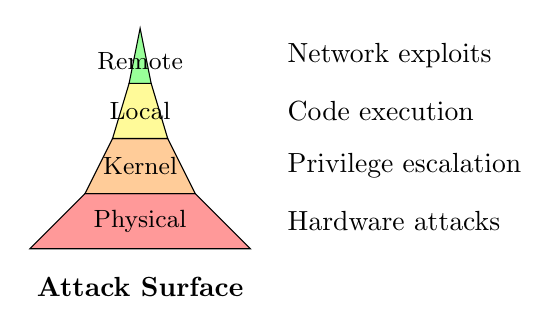
\begin{tikzpicture}[scale=0.7]
                % Threat levels pyramid
                \draw[fill=red!40] (0,0) -- (4,0) -- (3,1) -- (1,1) -- cycle;
                \node at (2,0.5) {\small Physical};
                
                \draw[fill=orange!40] (1,1) -- (3,1) -- (2.5,2) -- (1.5,2) -- cycle;
                \node at (2,1.5) {\small Kernel};
                
                \draw[fill=yellow!40] (1.5,2) -- (2.5,2) -- (2.2,3) -- (1.8,3) -- cycle;
                \node at (2,2.5) {\small Local};
                
                \draw[fill=green!40] (1.8,3) -- (2.2,3) -- (2,4) -- cycle;
                \node at (2,3.4) {\small Remote};
                
                % Labels
                \node[right] at (4.5,0.5) {Hardware attacks};
                \node[right] at (4.5,1.5) {Privilege escalation};
                \node[right] at (4.5,2.5) {Code execution};
                \node[right] at (4.5,3.5) {Network exploits};
                
                \node at (2,-0.7) {\textbf{Attack Surface}};
            \end{tikzpicture}
        \end{column}
    \end{columns}
    
    \vspace{0.5cm}
    \begin{tcolorbox}[colback=blue!10]
        \textbf{Modern CPU Security Mechanisms Target:}
        \begin{itemize}
            \item Memory corruption exploitation (buffer overflows, use-after-free)
            \item Control flow hijacking (ROP, JOP, code injection)
            \item Privilege escalation (kernel exploitation)
            \item Side-channel attacks (Spectre, Meltdown)
        \end{itemize}
    \end{tcolorbox}
\end{frame}

\begin{frame}{Defense in Depth}
    \begin{center}
        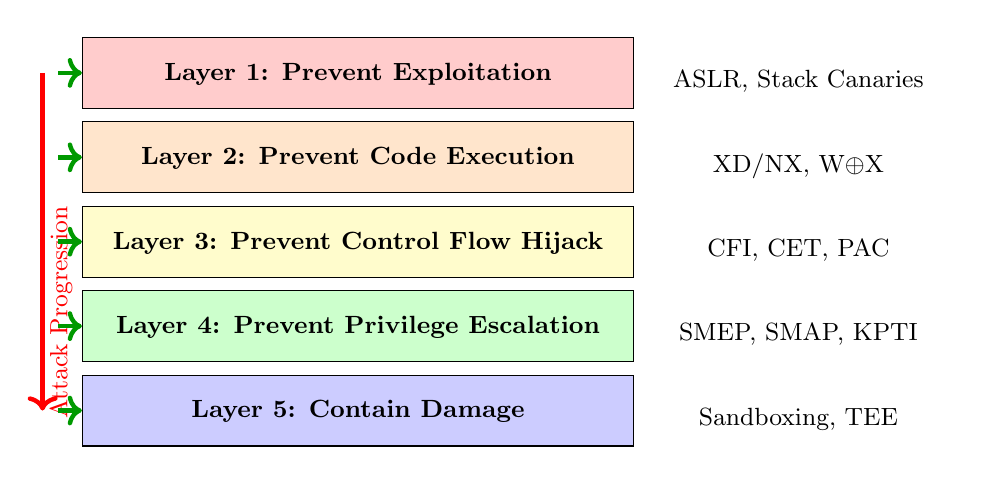
\begin{tikzpicture}[
            layer/.style={minimum height=0.9cm, text depth=0.2ex, font=\small},
            layer name/.style={layer, draw, minimum width=7cm},
            layer tech/.style={layer, minimum width=4cm, align=left, anchor=west}]

            \matrix[matrix of nodes, row sep=2pt, column sep=4pt,
                    ampersand replacement=\&, nodes={layer}] (m) {
                |[layer name, fill=red!20]| \textbf{Layer 1: Prevent Exploitation} \&
                |[layer tech]| ASLR, Stack Canaries \\
                |[layer name, fill=orange!20]| \textbf{Layer 2: Prevent Code Execution} \&
                |[layer tech]| XD/NX, W$\oplus$X \\
                |[layer name, fill=yellow!20]| \textbf{Layer 3: Prevent Control Flow Hijack} \&
                |[layer tech]| CFI, CET, PAC \\
                |[layer name, fill=green!20]| \textbf{Layer 4: Prevent Privilege Escalation} \&
                |[layer tech]| SMEP, SMAP, KPTI \\
                |[layer name, fill=blue!20]| \textbf{Layer 5: Contain Damage} \&
                |[layer tech]| Sandboxing, TEE \\
            };

            % Attack progression arrow - straight vertical line
            \draw[->, ultra thick, red] ([xshift=-0.5cm]m-1-1.west) -- ([xshift=-0.5cm]m-5-1.west);
            \node[rotate=90, red, font=\small, anchor=south, xshift=-0.9cm] at (m-3-1.west) {Attack Progression};

            % Defense arrows
            \foreach \i in {1,...,5} {
                \draw[<-, ultra thick, green!60!black] (m-\i-1.west) -- ++(-0.3,0);
            }
        \end{tikzpicture}
    \end{center}

    \vspace{0.3cm}
    \begin{tcolorbox}[colback=yellow!20]
        \centering
        \textbf{Principle:} No single defense is perfect - multiple independent layers increase attack complexity exponentially
    \end{tcolorbox}
\end{frame}

% Section: ROP Protection Evolution
\section{ROP Protection Evolution}

\begin{frame}{Execute Disable (XD/NX) Bit - The First Line}
    \begin{columns}
        \begin{column}{0.5\textwidth}
            \textbf{XD/NX Bit Basics:}
            \begin{itemize}
                \item Intel: XD (eXecute Disable)
                \item AMD: NX (No eXecute)
                \item ARM: XN (eXecute Never)
                \item Page table bit 63
            \end{itemize}
            
            \vspace{0.3cm}
            \textbf{How it Works:}
            \begin{itemize}
                \item Marks memory pages non-executable
                \item CPU raises \#PF on exec attempt
                \item Enforces W$\oplus$X policy
            \end{itemize}
        \end{column}
        \begin{column}{0.5\textwidth}
            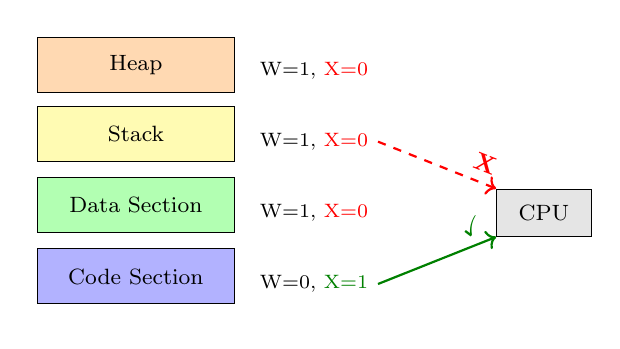
\begin{tikzpicture}[font=\footnotesize,
                mem section/.style={draw, minimum width=2.5cm, minimum height=0.7cm},
                perm/.style={minimum height=0.7cm, font=\scriptsize, anchor=west}]

                % Memory layout with permissions as second column
                \matrix[matrix of nodes, row sep=0.1cm, column sep=0.2cm,
                        ampersand replacement=\&] (mem) {
                    |[mem section, fill=orange!30]| Heap \&
                    |[perm]| W=1, \textcolor{red}{X=0} \\
                    |[mem section, fill=yellow!30]| Stack \&
                    |[perm]| W=1, \textcolor{red}{X=0} \\
                    |[mem section, fill=green!30]| Data Section \&
                    |[perm]| W=1, \textcolor{red}{X=0} \\
                    |[mem section, fill=blue!30]| Code Section \&
                    |[perm]| W=0, \textcolor{green!50!black}{X=1} \\
                };

                % CPU node
                \node[draw, fill=gray!20, minimum width=1.2cm, minimum height=0.6cm,
                      right=1.5cm of mem-3-2] (cpu) {CPU};

                % Execution arrow - only from Code Section (with checkmark)
                \draw[->, thick, green!50!black] (mem-4-2.east) -- (cpu.south west)
                    node[pos=0.85, above, font=\small, sloped] {\checkmark};

                % Blocked execution from Stack
                \draw[->, thick, red, dashed] (mem-2-2.east) -- (cpu.north west)
                    node[pos=0.85, above, font=\small\bfseries, sloped] {X};
            \end{tikzpicture}

            \vspace{0.3cm}
            \textbf{What XD Prevents:}
            \begin{itemize}
                \item Classic buffer overflow + shellcode
                \item Direct code injection attacks
            \end{itemize}
        \end{column}
    \end{columns}
\end{frame}

\begin{frame}[fragile]{Why XD/NX is Not Enough - Enter ROP}
    \begin{columns}
        \begin{column}{0.5\textwidth}
            \textbf{The Problem:}
            \begin{itemize}
                \item Attackers don't need new code!
                \item Existing code has everything needed
                \item Chain existing code snippets
            \end{itemize}
            
            \vspace{0.3cm}
            \textbf{Return-Oriented Programming:}
            \begin{itemize}
                \item Uses "gadgets" ending in RET
                \item Gadget = useful instruction(s) + RET
                \item Chain gadgets via stack control
                \item Turing complete!
            \end{itemize}
        \end{column}
        \begin{column}{0.5\textwidth}
            \begin{tcolorbox}[colback=gray!10]
                \small
                \textbf{ROP Attack Example:}
\begin{minted}[fontsize=\scriptsize]{nasm}
; Gadget 1: pop rdi; ret
; Gadget 2: pop rsi; ret
; Gadget 3: mov rax, 59; ret
; Gadget 4: syscall

Stack Layout:
[addr_gadget1]
["/bin/sh"]
[addr_gadget2]
[0]
[addr_gadget3]
[addr_gadget4]
\end{minted}
            \end{tcolorbox}
            
            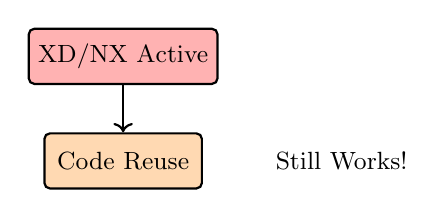
\begin{tikzpicture}[
                box/.style={draw, thick, minimum width=2cm, minimum height=0.7cm,
                           align=center, font=\small, rounded corners=2pt},
                arrow/.style={->, thick}]

                % XD/NX Active box at top
                \node[box, fill=red!30] (xd) {XD/NX Active};

                % Arrow pointing down
                \draw[arrow] (xd.south) -- ++(0, -0.6cm);

                % Code Reuse box below
                \node[box, fill=orange!30, below=0.6cm of xd] (reuse) {Code Reuse};

                % "Still Works!" annotation
                \node[font=\small, right=0.8cm of reuse] {Still Works!};
            \end{tikzpicture}
        \end{column}
    \end{columns}
\end{frame}

\begin{frame}{ROP Attack Visualization}
    \begin{center}
        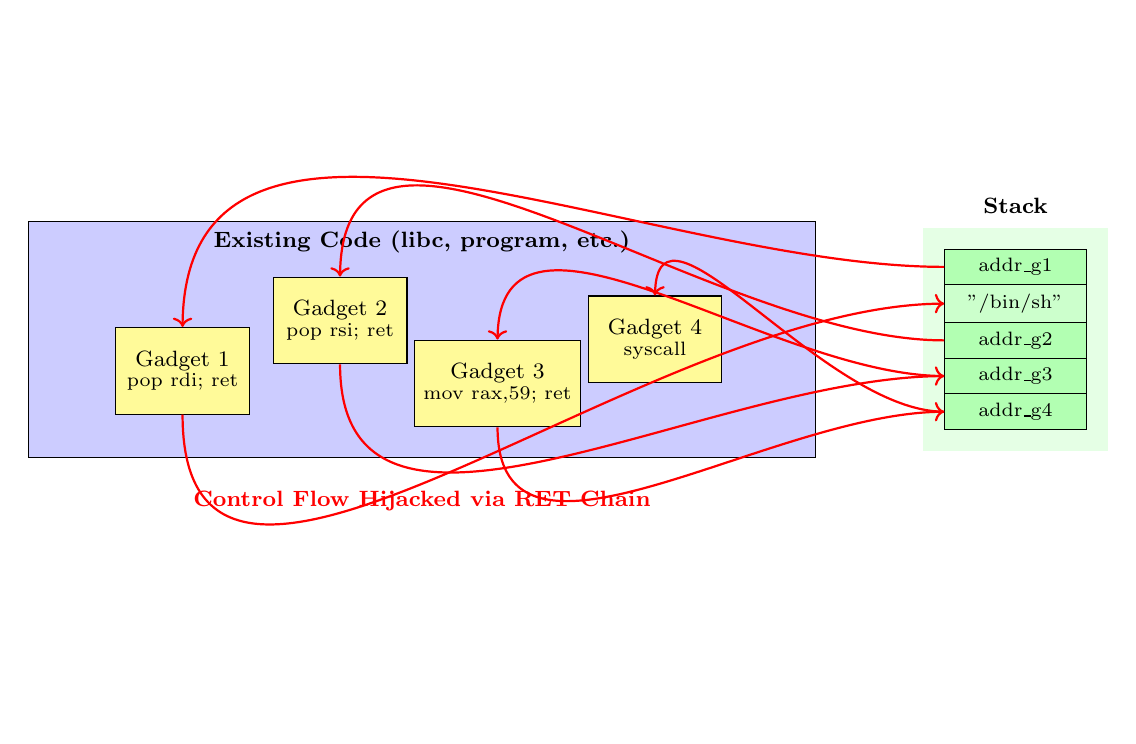
\begin{tikzpicture}[scale=0.8, font=\footnotesize,
            gadget/.style={draw, fill=yellow!40, minimum width=1.7cm, minimum height=1.1cm, align=center},
            stack cell/.style={draw, minimum width=1.8cm, minimum height=0.4cm, font=\scriptsize},
            flow/.style={->, thick, red}]

            % Code section background
            \node[draw, fill=blue!20, minimum width=10cm, minimum height=3cm] (code) at (5,1.5) {};
            \node[font=\footnotesize\bfseries, anchor=north] at (code.north) {Existing Code (libc, program, etc.)};

            % Gadgets - positioned within code section
            \node[gadget] (g1) at (1.2,1) {Gadget 1\\[-2pt]{\scriptsize pop rdi; ret}};
            \node[gadget] (g2) at (3.7,1.8) {Gadget 2\\[-2pt]{\scriptsize pop rsi; ret}};
            \node[gadget] (g3) at (6.2,0.8) {Gadget 3\\[-2pt]{\scriptsize mov rax,59; ret}};
            \node[gadget] (g4) at (8.7,1.5) {Gadget 4\\[-2pt]{\scriptsize syscall}};

            % Stack using matrix
            \matrix[matrix of nodes,
                nodes={stack cell},
                row sep=-\pgflinewidth,
                right=1.5cm of code] (stack) {
                |[fill=green!30]| addr\_g1 \\
                |[fill=green!20]| "/bin/sh" \\
                |[fill=green!30]| addr\_g2 \\
                |[fill=green!30]| addr\_g3 \\
                |[fill=green!30]| addr\_g4 \\
            };
            \node[font=\footnotesize\bfseries, above=0.2cm of stack] {Stack};

            % Background for stack
            \begin{scope}[on background layer]
                \node[fill=green!10, fit=(stack), inner sep=4pt] {};
            \end{scope}

            % Execution flow arrows
            \draw[flow] (stack-1-1.west) to[out=180,in=90] (g1.north);
            \draw[flow] (g1.south) to[out=-90,in=180] (stack-2-1.west);
            \draw[flow] (stack-3-1.west) to[out=180,in=90] (g2.north);
            \draw[flow] (g2.south) to[out=-90,in=180] (stack-4-1.west);
            \draw[flow] (stack-4-1.west) to[out=180,in=90] (g3.north);
            \draw[flow] (g3.south) to[out=-90,in=180] (stack-5-1.west);
            \draw[flow] (stack-5-1.west) to[out=180,in=90] (g4.north);

            % Caption
            \node[red, font=\footnotesize\bfseries, below=0.3cm of code] {Control Flow Hijacked via RET Chain};
        \end{tikzpicture}
    \end{center}

    \begin{tcolorbox}[colback=red!10]
        \textbf{Key Insight:} ROP bypasses XD/NX by reusing existing executable code - no code injection needed!
    \end{tcolorbox}
\end{frame}

% Protection Mechanisms in Detail
\begin{frame}[fragile]{ASLR - Address Space Layout Randomization}
    \begin{columns}
        \begin{column}{0.5\textwidth}
            \textbf{How ASLR Works:}
            \begin{itemize}
                \item Randomizes memory addresses at runtime
                \item Different addresses each execution
                \item Makes hardcoded exploits fail
                \item Low performance overhead
            \end{itemize}
            
            \vspace{0.3cm}
            \textbf{What Gets Randomized:}
            \begin{itemize}
                \item Stack base address
                \item Heap base address
                \item Library load addresses
                \item Executable base (PIE)
                \item mmap region
            \end{itemize}
            
            \vspace{0.3cm}
            \textbf{Limitations:}
            \begin{itemize}
                \item Info leaks reveal addresses
                \item Partial overwrites still work
                \item Entropy limitations (32-bit)
            \end{itemize}
        \end{column}
        \begin{column}{0.5\textwidth}
            \vspace{-3cm}
            \begin{tcolorbox}[colback=green!10]
                \small
                \textbf{With ASLR (randomized):}
\begin{minted}[fontsize=\scriptsize]{console}
$ ./vuln
Stack: 0x7ffd8c3a1000
Heap:  0x56412b8c9000
Libc:  0x7f9a2c600000

$ ./vuln
Stack: 0x7ffe29f43000
Heap:  0x55e7d4521000
Libc:  0x7fc8e1200000
\end{minted}
            \end{tcolorbox}
        \end{column}
    \end{columns}
\end{frame}

\begin{frame}[fragile]{Stack Canaries - Buffer Overflow Detection}
    \begin{columns}[T]
        \begin{column}{0.5\textwidth}
            \textbf{How Stack Canaries Work:}
            \begin{itemize}
                \item Random value placed before return address
                \item Checked before function returns
                \item Detects buffer overflows
                \item Compiler inserts automatically
            \end{itemize}
            
            \vspace{0.3cm}
            \textbf{Canary Types:}
            \begin{itemize}
                \item \textbf{Random:} From /dev/urandom
                \item \textbf{Terminator:} 0x00000aff
                \item \textbf{Random XOR:} Includes stack ptr
            \end{itemize}
        \end{column}
        \begin{column}{0.5\textwidth}
            \vspace{-7mm}
            \begin{tcolorbox}[colback=blue!10]
                \small
                \textbf{Vulnerable Function:}
\begin{minted}[fontsize=\scriptsize]{c}
void vulnerable(char *input) {
    char buffer[64];
    strcpy(buffer, input);
    return;
}
\end{minted}
            \end{tcolorbox}
            
            \begin{tcolorbox}[colback=green!10]
                \small
                \textbf{With Stack Canary:}
\begin{minted}[fontsize=\scriptsize]{nasm}
vulnerable:
    push rbp
    mov rbp, rsp
    sub rsp, 0x50

    ; Place canary
    mov rax, fs:[0x28]
    mov [rbp-0x8], rax

    ; Function body
    lea rdi, [rbp-0x48]
    call strcpy

    ; Check canary
    mov rax, [rbp-0x8]
    xor rax, fs:[0x28]
    jne .canary_fail

    leave
    ret

.canary_fail:
    call __stack_chk_fail
\end{minted}
            \end{tcolorbox}
        \end{column}
    \end{columns}
\end{frame}

\begin{frame}[fragile]{Stack Canary - Memory Layout}
    \begin{center}
        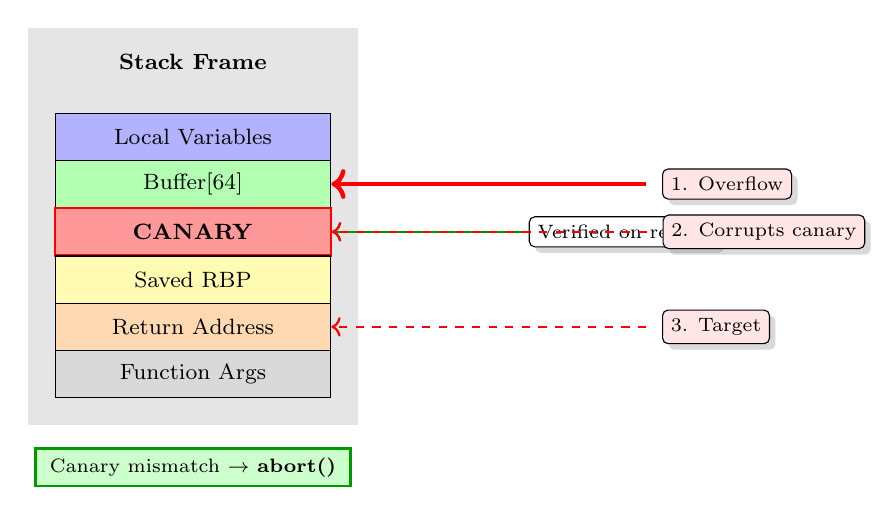
\begin{tikzpicture}[font=\footnotesize,
            stack cell/.style={draw, minimum width=3.5cm, minimum height=0.6cm},
            callout/.style={draw, fill=white, font=\scriptsize, rounded corners=2pt,
                           inner sep=3pt, drop shadow={opacity=0.3}}]

            % Stack frame title
            \node[font=\footnotesize\bfseries] (title) {Stack Frame};

            % Stack contents using matrix
            \matrix[matrix of nodes,
                nodes={stack cell},
                row sep=-\pgflinewidth,
                below=0.3cm of title] (stack) {
                |[fill=blue!30]| Local Variables \\
                |[fill=green!30]| Buffer[64] \\
                |[fill=red!40, draw=red, thick]| \textbf{CANARY} \\
                |[fill=yellow!30]| Saved RBP \\
                |[fill=orange!30]| Return Address \\
                |[fill=gray!30]| Function Args \\
            };

            % Background for stack frame
            \begin{scope}[on background layer]
                \node[fill=gray!20, fit=(title)(stack), inner sep=6pt] {};
            \end{scope}

            % Stage 1: Normal state - canary check annotation
            \node[callout, right=2.5cm of stack-3-1] (check) {Verified on return};
            \draw[->, thick, green!60!black] (check.west) -- (stack-3-1.east);

            % Stage 2: Overflow attack
            \onslide<2->{
                \draw[->, ultra thick, red] ([xshift=4cm]stack-2-1.east) -- (stack-2-1.east);
                \node[callout, fill=red!10, right=4.2cm of stack-2-1] (overflow) {1. Overflow};
            }

            % Stage 3: Canary corruption
            \onslide<3->{
                \draw[->, thick, red, dashed] ([xshift=4cm]stack-3-1.east) -- (stack-3-1.east);
                \node[callout, fill=red!10, right=4.2cm of stack-3-1] (corrupt) {2. Corrupts canary};
            }

            % Stage 4: Target and detection
            \onslide<4->{
                \draw[->, thick, red, dashed] ([xshift=4cm]stack-5-1.east) -- (stack-5-1.east);
                \node[callout, fill=red!10, right=4.2cm of stack-5-1] (target) {3. Target};
            }

            % Detection result
            \onslide<5->{
                \node[draw=green!60!black, fill=green!20, font=\scriptsize, thick,
                      below=0.5cm of stack, minimum width=4cm]
                    {Canary mismatch $\rightarrow$ \textbf{abort()}};
            }
        \end{tikzpicture}
    \end{center}
\end{frame}

% Section: SMEP and SMAP
\section{Kernel Protection: SMEP and SMAP}

\begin{frame}{SMEP - Supervisor Mode Execution Prevention}
    \begin{columns}
        \begin{column}{0.5\textwidth}
            \textbf{The Problem:}
            \begin{itemize}
                \item Kernel exploits redirect to user code
                \item User controls memory at known addresses
                \item ret2user attacks bypass KASLR
            \end{itemize}
            
            \vspace{0.3cm}
            \textbf{SMEP Solution:}
            \begin{itemize}
                \item CR4.SMEP bit (bit 20)
                \item Prevents kernel executing user pages
                \item \#PF if CPL=0 tries to execute U=1 page
                \item Intel: Ivy Bridge (2012)
            \end{itemize}
        \end{column}
        \begin{column}{0.5\textwidth}
            \begin{tikzpicture}[
                space/.style={draw, thick, minimum width=4cm, minimum height=2.5cm,
                            align=center, font=\small, rounded corners=2pt},
                label/.style={draw, fill=white, rounded corners=2pt, font=\tiny,
                            inner sep=2pt, align=center}]

                % Kernel Space at top
                \node[space, fill=purple!15] (kernel)
                    {\textbf{Kernel Space}};
                \node[label, below=2mm of kernel.north] (cpl0) {CPL = 0};
                \node[label, below=1mm of cpl0] {U = 0};

                % User Space below kernel
                \node[space, fill=cyan!10, below=1.2cm of kernel.south] (user)
                    {\textbf{User Space}};
                \node[label, below=2mm of user.north] (cpl3) {CPL = 3};
                \node[label, below=1mm of cpl3] (u1) {U = 1};
                \node[font=\small, below=1mm of u1, fill=red!20, rounded corners=2pt,
                      inner sep=2pt] {Shellcode};

                % Attack attempt with X mark
                \draw[->, thick, red, dashed] (kernel.south) -- ++(0, -0.5cm);
                \node[red, font=\small, left=2pt] at ([yshift=-2mm]kernel.south) {ret2user};
                \node[inner sep=0pt] at ([yshift=-5mm]kernel.south)
                    {\includegraphics[width=0.4cm]{figures/noun-x-2222229.png}};
                \node[red, font=\tiny, below=6mm of kernel.south] {SMEP Blocks!};

                % Consequence box
                \node[draw, fill=yellow!10, rounded corners=2pt, font=\tiny,
                      align=left, right=0.5cm of user.east, anchor=west, text width=2cm]
                    {\textbf{Without SMEP:}\\
                     Kernel jumps to\\
                     user shellcode\\
                     \textcolor{red}{= root shell}};
            \end{tikzpicture}
        \end{column}
    \end{columns}
    
    \vspace{0.3cm}
    \begin{tcolorbox}[colback=yellow!20]
        \textbf{Bypass Methods:} ROP in kernel code, physmap spraying, page table manipulation
    \end{tcolorbox}
\end{frame}

\begin{frame}[fragile]{SMAP - Supervisor Mode Access Prevention}
    \begin{columns}
        \begin{column}{0.5\textwidth}
            \textbf{The Problem After SMEP:}
            \begin{itemize}
                \item Can't execute user pages
                \item But can still READ/WRITE them!
                \item Kernel ROP can use user data
                \item Arbitrary write to user buffers
            \end{itemize}
            
            \vspace{0.3cm}
            \textbf{SMAP Solution:}
            \begin{itemize}
                \item CR4.SMAP bit (bit 21)
                \item Blocks kernel access to user pages
                \item STAC/CLAC instructions for legitimate access
                \item Intel: Broadwell (2014)
            \end{itemize}
        \end{column}
        \begin{column}{0.5\textwidth}
            \begin{tcolorbox}[colback=gray!10]
                \small
                \textbf{Kernel Code Pattern:}
\begin{minted}[fontsize=\scriptsize]{gas}
copy_from_user:
    STAC        ; Enable access
    mov (%rdi), %rax
    CLAC        ; Disable access
    ret

; Vulnerability example:
some_ioctl:
    ; Missing STAC/CLAC!
    mov %rsi, (%rdi)  ; Oops!
\end{minted}
            \end{tcolorbox}
            
            \textbf{EFLAGS.AC bit:}
            \begin{itemize}
                \item AC=0: SMAP active (default)
                \item AC=1: Temporary user access
                \item Only changeable in Ring 0
            \end{itemize}
        \end{column}
    \end{columns}
\end{frame}

\begin{frame}{SMEP + SMAP Combined Protection}
    \begin{center}
        \begin{tikzpicture}[
            space/.style={draw, thick, minimum width=8cm, minimum height=1.2cm,
                         align=center, font=\small},
            useritem/.style={draw, thick, minimum width=1.8cm, minimum height=0.8cm,
                           align=center, font=\small, rounded corners=2pt},
            attack/.style={->, thick, orange!70, dashed},
            allowed/.style={->, thick, green!60!black}]

            % Kernel Space at top - smaller and more compact
            \node[space, fill=purple!15, minimum height=0.9cm, text depth=3mm] (kernel) {\textbf{Kernel Space (Ring 0)}};

            % Protection barrier
            \coordinate (barrier-left) at ([xshift=-4cm]kernel.south);
            \coordinate (barrier-right) at ([xshift=4cm]kernel.south);
            \draw[ultra thick, red!70, dashed] (barrier-left) -- (barrier-right);
            \node[red!70, font=\small, right=2pt of barrier-right] {SMEP/SMAP};

            % User Space below barrier
            \node[space, fill=cyan!10, below=0.5cm of kernel.south] (user)
                {\textbf{User Space (Ring 3)}};

            % User components inside user space
            \node[useritem, fill=blue!20, above=0.2cm of user.south west, anchor=south west,
                  xshift=0.5cm] (code) {User Code};
            \node[useritem, fill=yellow!20, right=0.3cm of code] (data) {User Data};
            \node[useritem, fill=red!20, right=0.3cm of data] (rop) {ROP Chain};

            % Attack attempts from kernel
            \draw[attack] ([xshift=-2.5cm]kernel.south) -- ++(0, -0.4cm);
            \node[inner sep=0pt] at ([xshift=-2.5cm, yshift=-2mm]kernel.south)
                {\includegraphics[width=0.35cm]{figures/noun-x-2222229.png}};
            \node[orange!70, font=\tiny, above=1pt] at ([xshift=-2.5cm]kernel.south) {Execute};
            \node[red!70, font=\tiny, below=3mm] at ([xshift=-2.5cm]kernel.south) {SMEP};

            \draw[attack] ([xshift=-0.8cm]kernel.south) -- ++(0, -0.4cm);
            \node[inner sep=0pt] at ([xshift=-0.8cm, yshift=-2mm]kernel.south)
                {\includegraphics[width=0.35cm]{figures/noun-x-2222229.png}};
            \node[orange!70, font=\tiny, above=1pt] at ([xshift=-0.8cm]kernel.south) {Read};
            \node[red!70, font=\tiny, below=3mm] at ([xshift=-0.8cm]kernel.south) {SMAP};

            \draw[attack] ([xshift=0.8cm]kernel.south) -- ++(0, -0.4cm);
            \node[inner sep=0pt] at ([xshift=0.8cm, yshift=-2mm]kernel.south)
                {\includegraphics[width=0.35cm]{figures/noun-x-2222229.png}};
            \node[orange!70, font=\tiny, above=1pt] at ([xshift=0.8cm]kernel.south) {Write};
            \node[red!70, font=\tiny, below=3mm] at ([xshift=0.8cm]kernel.south) {SMAP};

            % Legitimate access with STAC
            \draw[allowed] ([xshift=2.5cm]kernel.south) -- ++(0, -0.4cm);
            \node[green!60!black, font=\tiny, above=1pt] at ([xshift=2.5cm]kernel.south) {STAC};
            \node[green!60!black, font=\small, below=2mm] at ([xshift=2.5cm]kernel.south) {$\checkmark$};
        \end{tikzpicture}
    \end{center}
    
    \vspace{0.3cm}
    \begin{columns}
        \begin{column}{0.5\textwidth}
            \textbf{Protection Matrix:}
            \begin{tabular}{|l|c|c|}
                \hline
                From Kernel & Execute & Access \\
                \hline
                No Protection & \checkmark & \checkmark \\
                SMEP only & $\times$ & \checkmark \\
                SMAP only & \checkmark & $\times$ \\
                SMEP+SMAP & $\times$ & $\times$* \\
                \hline
            \end{tabular}
            
            \small *Except with STAC/CLAC
        \end{column}
        \begin{column}{0.5\textwidth}
            \textbf{Remaining Attack Surface:}
            \begin{itemize}
                \item Kernel ROP/JOP only
                \item Kernel heap/stack spraying
                \item Race conditions in STAC/CLAC windows
                \item Hardware vulnerabilities (Spectre/Meltdown)
            \end{itemize}
        \end{column}
    \end{columns}
\end{frame}

\begin{frame}{Modern ROP Mitigations Summary}
    \begin{center}
        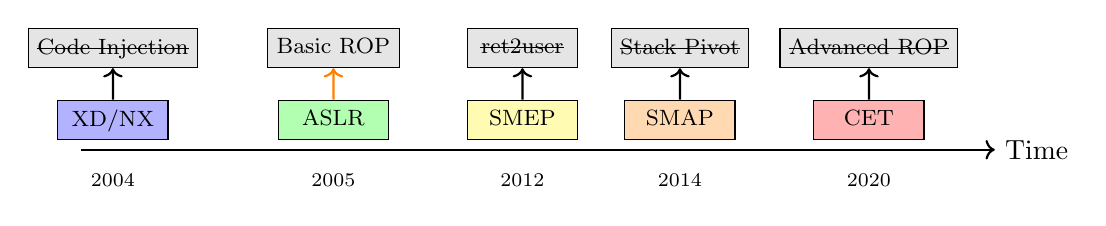
\begin{tikzpicture}[scale=0.8,
            year/.style={font=\scriptsize, text depth=0.25ex},
            defense/.style={draw, minimum width=1.4cm, minimum height=0.5cm, font=\footnotesize, text depth=0.25ex},
            attack/.style={draw, fill=gray!20, minimum width=1.4cm, minimum height=0.5cm, font=\footnotesize, text depth=0.25ex},
            mitigates/.style={->, thick},
            crossout/.style={thick, red}]

            % Timeline arrow - extended to avoid overlap with 2020
            \draw[thick,->] (-1.5,0) -- (13,0) node[right] {Time};

            % Year markers below the timeline
            \node[year] (y2004) at (-1,-0.5) {2004};
            \node[year] (y2005) at (2.5,-0.5) {2005};
            \node[year] (y2012) at (5.5,-0.5) {2012};
            \node[year] (y2014) at (8,-0.5) {2014};
            \node[year] (y2020) at (11,-0.5) {2020};

            % Defense nodes above timeline, aligned with years
            \node[defense, fill=blue!30, above=0.3cm of y2004] (nx) {XD/NX};
            \node[defense, fill=green!30, above=0.3cm of y2005] (aslr) {ASLR};
            \node[defense, fill=yellow!30, above=0.3cm of y2012] (smep) {SMEP};
            \node[defense, fill=orange!30, above=0.3cm of y2014] (smap) {SMAP};
            \node[defense, fill=red!30, above=0.3cm of y2020] (cet) {CET};

            % Attack nodes above defenses - close to the mechanism that stops them
            \node[attack, above=0.4cm of nx] (inject) {\sout{Code Injection}};
            \draw[mitigates] (nx) -- (inject);

            \node[attack, above=0.4cm of aslr] (rop) {Basic ROP};
            \draw[mitigates, orange] (aslr) -- (rop);

            \node[attack, above=0.4cm of smep] (ret2user) {\sout{ret2user}};
            \draw[mitigates] (smep) -- (ret2user);

            \node[attack, above=0.4cm of smap] (pivot) {\sout{Stack Pivot}};
            \draw[mitigates] (smap) -- (pivot);

            \node[attack, above=0.4cm of cet] (advanced) {\sout{Advanced ROP}};
            \draw[mitigates] (cet) -- (advanced);
        \end{tikzpicture}
    \end{center}
    
    \vspace{0.5cm}
    \begin{columns}
        \begin{column}{0.33\textwidth}
            \textbf{User Space:}
            \begin{itemize}
                \item XD/NX bit
                \item ASLR
                \item Stack Canaries
                \item CFI/CET
                \item Shadow Stack
            \end{itemize}
        \end{column}
        \begin{column}{0.33\textwidth}
            \textbf{Kernel Space:}
            \begin{itemize}
                \item SMEP (HW)
                \item SMAP (HW)
                \item KASLR (SW)
                \item KPTI* (SW)
                \item FineIBT (HW+SW)
            \end{itemize}
        \end{column}
        \begin{column}{0.33\textwidth}
            \textbf{Hardware:}
            \begin{itemize}
                \item Intel CET
                \item ARM PAC/BTI
                \item ARM MTE
                \item Control-flow integrity
            \end{itemize}
        \end{column}
    \end{columns}
    
    \vspace{0.2cm}
    \small *KPTI: Kernel Page Table Isolation - software mitigation for Meltdown
\end{frame}

\begin{frame}{Performance Impact of Security Features}
    \begin{center}
        \begin{tabular}{|l|c|c|l|}
            \hline
            \textbf{Feature} & \textbf{Type} & \textbf{Impact} & \textbf{Overhead} \\
            \hline
            \hline
            XD/NX Bit & HW & \cellcolor{green!30}Low & Page table bit check \\
            \hline
            SMEP & HW & \cellcolor{green!30}Low & Permission check \\
            \hline
            SMAP & HW & \cellcolor{green!30}Low & AC flag check \\
            \hline
            Stack Canaries & SW & \cellcolor{green!30}Low & Function epilogue check \\
            \hline
            ASLR & SW & \cellcolor{green!30}Low & One-time randomization \\
            \hline
            CET (Shadow Stack) & HW & \cellcolor{yellow!30}Medium & Parallel stack ops \\
            \hline
            PAC (ARM) & HW & \cellcolor{yellow!30}Medium & Crypto ops per call \\
            \hline
            BTI (ARM) & HW & \cellcolor{yellow!30}Medium & Branch checks \\
            \hline
            KASLR & SW & \cellcolor{yellow!30}Medium & Kernel relocation \\
            \hline
            KPTI* & SW & \cellcolor{orange!30}High & Page table switches \\
            \hline
            Full CFI** & SW & \cellcolor{orange!30}High & Type checks everywhere \\
            \hline
            FineIBT & HW+SW & \cellcolor{yellow!30}Medium & Hash + branch checks \\
            \hline
        \end{tabular}
    \end{center}
    
    \vspace{0.3cm}
    \begin{columns}
        \begin{column}{0.5\textwidth}
            \small
            *Software mitigation for Meltdown\\
            **Software-only implementation
        \end{column}
        \begin{column}{0.5\textwidth}
            \begin{tcolorbox}[colback=yellow!10]
                \small
                \textbf{Impact Categories:}
                \begin{itemize}
                    \item \textcolor{green!70!black}{Low}: $<$5\%
                    \item \textcolor{yellow!70!black}{Medium}: 5-15\%
                    \item \textcolor{orange!70!black}{High}: $>$15\%
                \end{itemize}
            \end{tcolorbox}
        \end{column}
    \end{columns}
\end{frame}

% Section 1: Memory Protection
\section{Memory Protection Mechanisms}

\begin{frame}{Pointer Tagging}
    \begin{columns}
        \begin{column}{0.5\textwidth}
            \textbf{Concept:}
            \begin{itemize}
                \item Uses unused bits in 64-bit pointers
                \item Tags store metadata (type, color, version)
                \item Enables memory safety checks
            \end{itemize}
            
            \vspace{0.5cm}
            \textbf{Benefits:}
            \begin{itemize}
                \item Detect use-after-free
                \item Prevent type confusion
                \item Low overhead ($<$5\%)
            \end{itemize}
        \end{column}
        \begin{column}{0.5\textwidth}
            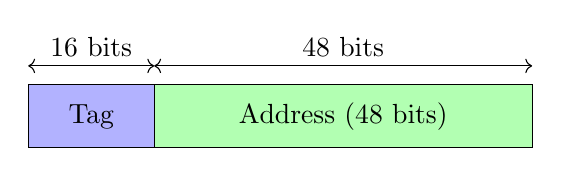
\begin{tikzpicture}[scale=0.8]
                \draw (0,0) rectangle (8,1);
                \draw[fill=blue!30] (0,0) rectangle (2,1);
                \draw[fill=green!30] (2,0) rectangle (8,1);
                \node at (1,0.5) {Tag};
                \node at (5,0.5) {Address (48 bits)};
                \draw[<->] (0,1.3) -- (2,1.3) node[midway,above] {16 bits};
                \draw[<->] (2,1.3) -- (8,1.3) node[midway,above] {48 bits};
            \end{tikzpicture}
            
            \vspace{0.5cm}
            \textbf{Example: ARM MTE}
            \begin{itemize}
                \item 4-bit tags in bits [59:56]
                \item Hardware tag checking
                \item Synchronous/async exceptions
            \end{itemize}
        \end{column}
    \end{columns}
\end{frame}

\begin{frame}[fragile]{ARM MTE - How It Works}
    \begin{columns}
        \begin{column}{0.5\textwidth}
            \textbf{Memory Granularity:}
            \begin{itemize}
                \item Each 16-byte memory granule has a 4-bit tag
                \item Tags stored in dedicated tag memory
                \item Tag memory not directly accessible
            \end{itemize}

            %\vspace{0.3cm}
            \textbf{Hardware Tag Checking:}
            \begin{itemize}
                \item On every load/store: compare pointer tag with memory tag
                \item If mismatch $\rightarrow$ exception
                \item Synchronous or asynchronous mode
            \end{itemize}

            %\vspace{0.3cm}
            \textbf{Software Behavior:}
            \begin{itemize}
                \item \texttt{malloc()}: assigns random tag to allocation
                \item \texttt{free()}: changes memory tag
                \item Old pointers become invalid
            \end{itemize}
        \end{column}
        \begin{column}{0.5\textwidth}
            \vspace{-3mm}
            \begin{tcolorbox}[colback=gray!10, left=1mm, right=1mm, top=1mm, bottom=1mm]
\begin{minted}[fontsize=\footnotesize]{c}
// Allocation - tag = 0x5
char *ptr = malloc(64);
// ptr = 0x5_00001000 (tag bits 59:56)
// Memory at 0x1000 tagged with 0x5

strcpy(ptr, "hello");  // OK: tags match

free(ptr);  // Memory retagged to 0x7
            // ptr still has tag 0x5

// Use-after-free attempt:
strcpy(ptr, "bad");  // EXCEPTION!
// ptr tag (0x5) != memory tag (0x7)
\end{minted}
            \end{tcolorbox}

            \vspace{0.1cm}
            {\tiny Note: Tags are random, not sequential}
        \end{column}
    \end{columns}
\end{frame}

\begin{frame}{ARM MTE in Action}
    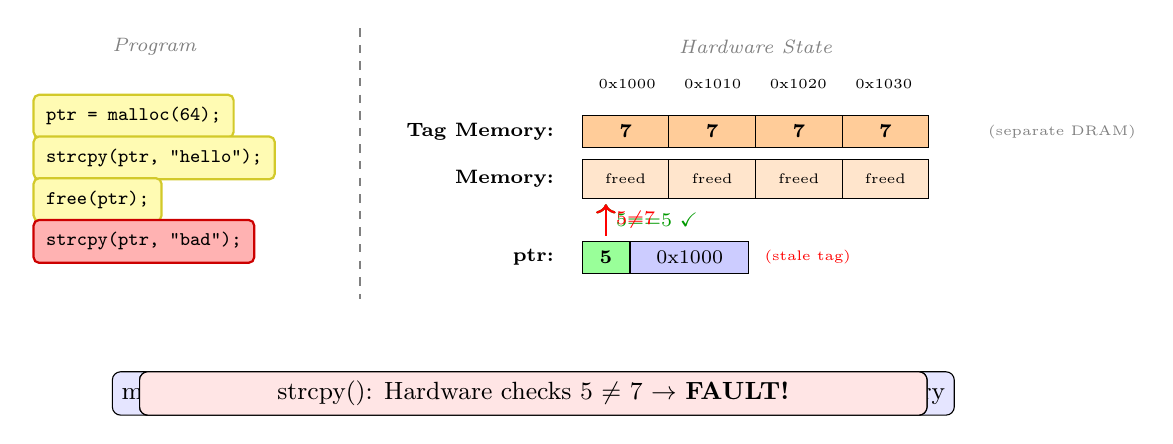
\begin{tikzpicture}[
        memcell/.style={draw, minimum width=1.1cm, minimum height=0.5cm, font=\tiny},
        tagcell/.style={draw, minimum width=1.1cm, minimum height=0.4cm, font=\scriptsize\bfseries},
        codeline/.style={font=\ttfamily\scriptsize, anchor=west},
        highlight/.style={draw=yellow!80!black, fill=yellow!30, thick, rounded corners=2pt},
        highlight bad/.style={draw=red!80!black, fill=red!30, thick, rounded corners=2pt},
        rowlabel/.style={font=\scriptsize\bfseries, anchor=east},
        ptrtag/.style={draw, minimum width=0.6cm, minimum height=0.4cm, font=\scriptsize\bfseries},
        ptrval/.style={draw, minimum width=1.5cm, minimum height=0.4cm, font=\scriptsize},
        allocated/.style={fill=green!40},
        freed/.style={fill=orange!40},
        allocmem/.style={fill=green!20},
        freedmem/.style={fill=orange!20},
        result/.style={draw=red, fill=red!20, thick, font=\small\bfseries, rounded corners=3pt}]

        % Code listing (left side)
        \matrix[matrix of nodes, nodes={codeline}, row sep=2pt] (code) {
            |(c1)| ptr = malloc(64); \\
            |(c2)| strcpy(ptr, "hello"); \\
            |(c3)| free(ptr); \\
            |(c4)| strcpy(ptr, "bad"); \\
        };

        % Highlight current line (on background layer so code stays visible)
        \begin{scope}[on background layer]
            \onslide<2>{\node[highlight, fit=(c1), inner sep=1pt] {};}
            \onslide<3>{\node[highlight, fit=(c2), inner sep=1pt] {};}
            \onslide<4>{\node[highlight, fit=(c3), inner sep=1pt] {};}
            \onslide<5-6>{\node[highlight bad, fit=(c4), inner sep=1pt] {};}
        \end{scope}

        % Right side - memory visualization
        % Tag Memory (separate storage) with address labels above
        \node[rowlabel] (taglabel) at (5.2, 0.6) {Tag Memory:};
        \matrix[matrix of nodes,
            nodes={tagcell, fill=gray!20},
            column sep=-\pgflinewidth,
            ampersand replacement=\&,
            right=3pt of taglabel.east, anchor=west] (tags) {
            - \& - \& - \& - \\
        };
        % Address labels above tag cells (no border/background)
        \matrix[matrix of nodes,
            nodes={font=\tiny, minimum width=1.1cm, minimum height=0.3cm, inner sep=0pt},
            column sep=-\pgflinewidth,
            ampersand replacement=\&,
            anchor=south] at (tags.north) {
            0x1000 \& 0x1010 \& 0x1020 \& 0x1030 \\
        };

        % Color the tag cells based on state
        \onslide<2-3>{
            \node[tagcell, allocated] at (tags-1-1) {5};
            \node[tagcell, allocated] at (tags-1-2) {5};
            \node[tagcell, allocated] at (tags-1-3) {5};
            \node[tagcell, allocated] at (tags-1-4) {5};
        }
        \onslide<4->{
            \node[tagcell, freed] at (tags-1-1) {7};
            \node[tagcell, freed] at (tags-1-2) {7};
            \node[tagcell, freed] at (tags-1-3) {7};
            \node[tagcell, freed] at (tags-1-4) {7};
        }

        % Main Memory - label aligned to taglabel, matrix aligned to tags
        \node[rowlabel, below=0.6cm of taglabel.east, anchor=east] (memlabel) {Memory:};
        \matrix[matrix of nodes,
            nodes={memcell, fill=gray!10},
            column sep=-\pgflinewidth,
            ampersand replacement=\&,
            anchor=west] (mem) at (tags.west |- memlabel) {
            --- \& --- \& --- \& --- \\
        };

        % Color memory based on state - show content, not addresses
        \onslide<2>{
            \node[memcell, allocmem] at (mem-1-1) {---};
            \node[memcell, allocmem] at (mem-1-2) {---};
            \node[memcell, allocmem] at (mem-1-3) {---};
            \node[memcell, allocmem] at (mem-1-4) {---};
        }
        \onslide<3>{
            \node[memcell, allocmem] at (mem-1-1) {"hel};
            \node[memcell, allocmem] at (mem-1-2) {lo"};
            \node[memcell, allocmem] at (mem-1-3) {---};
            \node[memcell, allocmem] at (mem-1-4) {---};
        }
        \onslide<4->{
            \node[memcell, freedmem] at (mem-1-1) {freed};
            \node[memcell, freedmem] at (mem-1-2) {freed};
            \node[memcell, freedmem] at (mem-1-3) {freed};
            \node[memcell, freedmem] at (mem-1-4) {freed};
        }

        % Pointer variable - label aligned to memlabel, larger gap from Memory row
        \node[rowlabel, below=1cm of memlabel.east, anchor=east] (ptrlabel) {ptr:};
        \node[ptrtag, fill=gray!20, anchor=west] (ptrtag-node) at (mem-1-1.west |- ptrlabel) {-};
        \node[ptrval, fill=gray!10, anchor=west] (ptrval-node) at (ptrtag-node.east) {NULL};

        % Update pointer on malloc - positioned relative to mem-1-1 and ptrtag-alloc
        \onslide<2->{
            \node[ptrtag, allocated, anchor=west] (ptrtag-alloc) at (mem-1-1.west |- ptrlabel) {5};
            \node[ptrval, fill=blue!20, anchor=west] (ptrval-alloc) at (ptrtag-alloc.east) {0x1000};
        }
        \onslide<4->{
            \node[font=\tiny, red, right=2pt of ptrval-alloc.east] {(stale tag)};
        }

        % Tag comparison visualization
        \onslide<3>{
            \draw[->, thick, green!60!black] ([yshift=2pt]ptrtag-alloc.north) -- ++(0, 0.4)
                node[right, font=\scriptsize, pos=0.5] {5==5 \checkmark};
        }
        \onslide<5->{
            \draw[->, thick, red] ([yshift=2pt]ptrtag-alloc.north) -- ++(0, 0.4)
                node[right, font=\scriptsize, pos=0.5] {5$\neq$7};
        }

        % Labels for sections
        \node[font=\scriptsize\itshape, gray, above=0.3cm of code.north] (proglabel) {Program};
        \node[font=\scriptsize\itshape, gray] at (tags.north |- proglabel) {Hardware State};

        % Separator line - from above program label to below ptr
        \draw[gray, dashed] ([xshift=1cm]proglabel.north -| code.east) -- ([xshift=1cm, yshift=-0.3cm]ptrlabel.south -| code.east);

        % Note about tag memory
        \node[font=\tiny, gray, anchor=west] at ([xshift=0.5cm]tags.east) {(separate DRAM)};

        % Description box at bottom center - use separate overlaid nodes
        \coordinate (descpos) at ([yshift=-1.5cm]ptrlabel.south);
        \onslide<1>{\node[draw, fill=blue!10, rounded corners=3pt, font=\small, minimum width=10cm] at (descpos) {Initial state: pointer is NULL, memory unallocated};}
        \onslide<2>{\node[draw, fill=blue!10, rounded corners=3pt, font=\small, minimum width=10cm] at (descpos) {malloc(64): Allocates memory, assigns tag 5 to both pointer and memory};}
        \onslide<3>{\node[draw, fill=green!10, rounded corners=3pt, font=\small, minimum width=10cm] at (descpos) {strcpy(): Hardware checks pointer tag (5) == memory tag (5) \checkmark};}
        \onslide<4>{\node[draw, fill=orange!10, rounded corners=3pt, font=\small, minimum width=10cm] at (descpos) {free(): Memory tag changed to 7, but pointer still has tag 5};}
        \onslide<5-6>{\node[draw, fill=red!10, rounded corners=3pt, font=\small, minimum width=10cm] at (descpos) {strcpy(): Hardware checks 5 $\neq$ 7 $\rightarrow$ \textbf{FAULT!}};}
    \end{tikzpicture}
\end{frame}

\begin{frame}[fragile]{Pointer Authentication (PAC)}
    \begin{columns}
        \begin{column}{0.5\textwidth}
            \textbf{ARM PAC Architecture:}
            \begin{itemize}
                \item Cryptographic signature in pointer
                \item Uses QARMA block cipher
                \item 5 128-bit keys (IA, IB, DA, DB, GA)
            \end{itemize}
            
            \vspace{0.3cm}
            \textbf{Operations:}
            \begin{itemize}
                \item \texttt{PACIA}: Sign instruction pointer
                \item \texttt{AUTIA}: Authenticate pointer
                \item \texttt{PACDA}: Sign data pointer
            \end{itemize}
        \end{column}
        \begin{column}{0.5\textwidth}
            \begin{tcolorbox}[colback=gray!10]
                \small
                \textbf{Function Prologue:}
\begin{minted}[fontsize=\scriptsize]{gas}
PACIASP    ; Sign LR with SP
STP x29,x30,[sp,#-16]!
\end{minted}

                \textbf{Function Epilogue:}
\begin{minted}[fontsize=\scriptsize]{gas}
LDP x29,x30,[sp],#16
AUTIASP    ; Verify LR
RET        ; Return if valid
\end{minted}
            \end{tcolorbox}
            
            \vspace{0.2cm}
            \textbf{Key Terms:}
            \begin{itemize}
                \item \textbf{LR (x30):} Link Register - stores return address
                \item \textbf{SP:} Stack Pointer - used as context
                \item \textbf{x29:} Frame Pointer
            \end{itemize}
            
            \textbf{Security:} Prevents ROP/JOP attacks
        \end{column}
    \end{columns}
\end{frame}

% Section 2: Control Flow Integrity
\section{Control Flow Integrity}

\begin{frame}{Control Flow Integrity (CFI) - Overview}
    \begin{columns}
        \begin{column}{0.5\textwidth}
            \textbf{Core Concept:}
            \begin{itemize}
                \item Enforce legitimate control flow transfers
                \item Prevent code-reuse attacks (ROP/JOP/COP)
                \item Hardware + software enforcement
            \end{itemize}
            
            \vspace{0.3cm}
            \textbf{Two Protection Categories:}
            
            \colorbox{green!20}{\textbf{Forward-Edge CFI:}}
            \begin{itemize}
                \item Indirect calls (call rax)
                \item Indirect jumps (jmp rbx)
                \item Virtual function calls
            \end{itemize}
            
            \colorbox{blue!20}{\textbf{Backward-Edge CFI:}}
            \begin{itemize}
                \item Function returns (ret)
                \item Return address integrity
            \end{itemize}
        \end{column}
        \begin{column}{0.5\textwidth}
            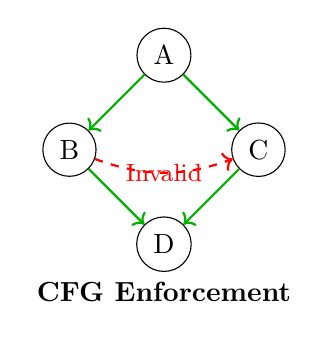
\begin{tikzpicture}[scale=0.6]
                % Control flow graph
                \node[draw,circle] (A) at (2,4) {A};
                \node[draw,circle] (B) at (0,2) {B};
                \node[draw,circle] (C) at (4,2) {C};
                \node[draw,circle] (D) at (2,0) {D};
                
                % Valid edges (green)
                \draw[->,thick,green!70!black] (A) -- (B);
                \draw[->,thick,green!70!black] (A) -- (C);
                \draw[->,thick,green!70!black] (B) -- (D);
                \draw[->,thick,green!70!black] (C) -- (D);
                
                % Invalid edge (red, dashed)
                \draw[->,thick,red,dashed] (B) to[bend right=20] (C);
                \node[red] at (2,1.5) {\small Invalid};
                
                \node at (2,-1) {\textbf{CFG Enforcement}};
            \end{tikzpicture}
            
            \vspace{0.3cm}
            \begin{tcolorbox}[colback=yellow!10]
                \small
                \textbf{Attack Example:}
                Attacker overwrites function pointer to jump from B→C, violating intended control flow
            \end{tcolorbox}
        \end{column}
    \end{columns}
\end{frame}

\begin{frame}[fragile]{Forward-Edge CFI Mechanisms}
    \begin{columns}
        \begin{column}{0.5\textwidth}
            \textbf{Intel CET-IBT (Indirect Branch Tracking):}
            \begin{itemize}
                \item \texttt{ENDBRANCH} instruction marks valid targets
                \item CPU tracks indirect branch state
                \item Fault if target lacks \texttt{ENDBRANCH}
            \end{itemize}
            
            \vspace{0.3cm}
            \textbf{ARM BTI (Branch Target Identification):}
            \begin{itemize}
                \item \texttt{BTI} instructions mark valid targets
                \item Variants match branch types:
                \begin{itemize}
                    \item \texttt{BTI c}: Call target (BLR)
                    \item \texttt{BTI j}: Jump target (BR)
                    \item \texttt{BTI jc}: Both call \& jump
                \end{itemize}
                \item CPU faults on mismatch
            \end{itemize}
            
            \vspace{0.3cm}
            \textbf{Software CFI (LLVM):}
            \begin{itemize}
                \item Type-based: Check function signatures
                \item Fine-grained: Unique IDs per callsite
                \item Cross-DSO support
            \end{itemize}
        \end{column}
        \begin{column}{0.5\textwidth}
            \begin{tcolorbox}[colback=gray!10]
                \small
                \textbf{Example: Intel CET-IBT}
\begin{minted}[fontsize=\scriptsize]{nasm}
valid_target:
    endbranch    ; Mark as valid
    push rbp
    mov rbp, rsp
    ; Function body

invalid_target:  ; No endbranch
    push rbp     ; CPU fault here!
    mov rbp, rsp
\end{minted}
            \end{tcolorbox}
            
            \textbf{Protection Granularity:}
            \begin{itemize}
                \item \textbf{Coarse:} Any valid function
                \item \textbf{Fine:} Type-compatible functions
                \item \textbf{Ultra-fine:} Exact callsite matching
            \end{itemize}
        \end{column}
    \end{columns}
\end{frame}

\begin{frame}[fragile]{ARM BTI Explained}
    \begin{columns}
        \begin{column}{0.5\textwidth}
            \textbf{BTI Instruction Variants:}
            \begin{itemize}
                \item \textbf{BTI c}: Target of calls (BLR/BLRA)
                \item \textbf{BTI j}: Target of jumps (BR/BRA)
                \item \textbf{BTI jc}: Target of both
                \item \textbf{BTI}: Same as BTI jc (alias)
            \end{itemize}
            
            \vspace{0.3cm}
            \textbf{How It Works:}
            \begin{enumerate}
                \item Indirect branch sets PSTATE.BTYPE
                \item Target instruction checked
                \item Must be correct BTI variant
                \item Otherwise: exception generated
            \end{enumerate}
            
            \vspace{0.3cm}
            \textbf{Use Cases:}
            \begin{itemize}
                \item Function entry points: BTI c
                \item Switch jump tables: BTI j
                \item PLT stubs: BTI jc
            \end{itemize}
        \end{column}
        \begin{column}{0.5\textwidth}
            \vspace{-7mm}
            \begin{tcolorbox}[colback=gray!10]
                \small
                \textbf{BTI Usage Example:}
\begin{minted}[fontsize=\scriptsize]{gas}
; Function called via pointer
func_ptr:
    BTI c      ; Mark as call target
    stp x29, x30, [sp, #-16]!
    ; Function body
    ldp x29, x30, [sp], #16
    ret

; Jump table target
case_handler:
    BTI j      ; Mark as jump target
    ; Handle case
    ret

; PLT stub (can be called or jumped to)
plt_stub:
    BTI jc     ; Both call and jump
    adrp x16, GOT_ENTRY
    ldr x17, [x16, #:lo12:GOT_ENTRY]
    br x17
\end{minted}
            \end{tcolorbox}
        \end{column}
    \end{columns}
\end{frame}

\begin{frame}[fragile]{Pointer Authentication (PAC) - ARM64}
    \begin{columns}
        \begin{column}{0.5\textwidth}
            \textbf{How PAC Works:}
            \begin{itemize}
                \item Signs pointers with cryptographic MAC
                \item Uses upper bits (unused in 64-bit)
                \item Hardware acceleration (QARMA)
                \item 5 different keys (IA, IB, DA, DB, GA)
            \end{itemize}
            
            \vspace{0.3cm}
            \textbf{PAC Instructions:}
            \begin{itemize}
                \item \textbf{PACIA:} Sign with key A
                \item \textbf{AUTIA:} Authenticate with key A
                \item \textbf{PACIASP:} Sign with SP as context
                \item \textbf{AUTIASP:} Auth with SP as context
            \end{itemize}
            
            \vspace{0.3cm}
            \textbf{Protection Against:}
            \begin{itemize}
                \item ROP/JOP attacks
                \item Return address corruption
                \item Function pointer hijacking
            \end{itemize}
        \end{column}
        \begin{column}{0.5\textwidth}
            \vspace{-7mm}
            \begin{tcolorbox}[colback=green!10, left=1mm, right=1mm, top=1mm, bottom=1mm]
\begin{minted}[fontsize=\scriptsize]{gas}
sensitive_function:
    paciasp          ; Sign return address
    ; Save frame
    stp x29, x30, [sp, #-16]!
    mov x29, sp
    ; Function body ...
    ; Restore frame
    ldp x29, x30, [sp], #16
    ; Authenticate return address
    autiasp
    ; Return (crashes if auth fails)
    ret
\end{minted}
            \end{tcolorbox}

            \begin{tcolorbox}[colback=yellow!10]
                \small
                \textbf{Pointer Format:}
\begin{minted}[fontsize=\scriptsize]{text}
[63:56][55:48][47:0]
  PAC   Unused  Address
\end{minted}
            \end{tcolorbox}
        \end{column}
    \end{columns}
\end{frame}

\begin{frame}[fragile]{Shadow Stack - Hardware Return Address Protection}
    \begin{columns}
        \begin{column}{0.5\textwidth}
            \textbf{Shadow Stack Concept:}
            \begin{itemize}
                \item Separate stack for return addresses
                \item Write-protected by hardware
                \item Parallel push/pop operations
                \item Automatic verification on return
            \end{itemize}
            
            \vspace{0.3cm}
            \textbf{Intel CET Implementation:}
            \begin{itemize}
                \item New SSP register (Shadow Stack Pointer)
                \item WRSS/RDSS instructions (privileged)
                \item Automatic on CALL/RET
                \item Page table bit for SS pages
            \end{itemize}
            
            \vspace{0.3cm}
            \textbf{Benefits:}
            \begin{itemize}
                \item Complete ROP prevention
                \item Zero false positives
                \item Hardware speed
                \item Transparent to applications
            \end{itemize}
        \end{column}
        \begin{column}{0.5\textwidth}
            \vspace{-7mm}
            \begin{tikzpicture}[font=\scriptsize,
                stack title/.style={font=\scriptsize\bfseries},
                stack cell/.style={draw, minimum width=2cm, minimum height=0.5cm, anchor=north, inner sep=2pt},
                stack container/.style={draw, fill=#1, rounded corners=2pt},
                stack container/.default=blue!20]

                % Regular Stack using matrix
                \matrix[matrix of nodes,
                    nodes={stack cell},
                    row sep=-\pgflinewidth,
                    column sep=0pt] (regstack) {
                    |[fill=gray!20]| Local Vars \\
                    |[fill=yellow!30]| Return Addr \\
                    |[fill=gray!20]| Saved RBP \\
                };
                \node[stack title, above=0.15cm of regstack] {Regular Stack};
                \begin{scope}[on background layer]
                    \node[stack container=blue!20, fit=(regstack), inner sep=2pt] {};
                \end{scope}

                % Shadow Stack using matrix
                \matrix[matrix of nodes,
                    nodes={stack cell},
                    row sep=-\pgflinewidth,
                    right=1.3cm of regstack] (shadowstack) {
                    |[fill=green!40]| Return Addr \\
                };
                \node[stack title, above=0.15cm of shadowstack] {Shadow Stack};
                \begin{scope}[on background layer]
                    \node[stack container=green!20, draw=green!60!black, thick,
                          fit=(shadowstack), inner sep=2pt] {};
                \end{scope}

                % Protection label
                \node[draw, fill=red!20, font=\scriptsize, below=0.5cm of shadowstack] (prot) {Write Protected};

                % Verify arrow between return addresses
                \draw[<->, thick] (regstack-2-1.east) -- (shadowstack-1-1.west)
                    node[midway, above, font=\scriptsize] {Verify};

                % Attack arrow
                \draw[->, thick, red] ([xshift=-1cm]regstack-2-1.west) -- (regstack-2-1.west)
                    node[midway, above, font=\scriptsize] {Overflow};

                % X mark for blocked access
                \node[inner sep=0pt, right=0.3cm of shadowstack-1-1.east]
                    {\includegraphics[width=0.4cm]{figures/noun-x-2222229.png}};
            \end{tikzpicture}
            
            \vspace{0.3cm}
            \begin{tcolorbox}[colback=yellow!10]
                \small
                \textbf{Operation Example:}
\begin{minted}[fontsize=\scriptsize]{text}
CALL func:
  - Push addr to regular stack
  - Push addr to shadow stack

RET:
  - Pop from regular stack -> RAX
  - Pop from shadow stack -> RBX
  - If RAX != RBX -> Fault
\end{minted}
            \end{tcolorbox}
        \end{column}
    \end{columns}
\end{frame}

\begin{frame}[fragile]{The Type Confusion Problem}
    \begin{columns}
        \begin{column}{0.5\textwidth}
            \textbf{What is Type Confusion?}
            \begin{itemize}
                \item Object interpreted as wrong type
                \item Common in C++ with inheritance
                \item Enables control flow hijacking
                \item Bypass basic CFI checks
            \end{itemize}
            
            \vspace{0.3cm}
            \textbf{Attack Scenario:}
            \begin{itemize}
                \item Attacker controls object allocation
                \item Forces type confusion via UAF/overflow
                \item Calls virtual function on wrong type
                \item Jumps to attacker-controlled vtable
            \end{itemize}
            
            \vspace{0.3cm}
            \textbf{Why Basic CFI Fails:}
            \begin{itemize}
                \item All virtual calls are "valid" targets
                \item Cannot distinguish object types
                \item Need type-aware CFI (FineIBT)
            \end{itemize}
        \end{column}
        \begin{column}{0.5\textwidth}
            \begin{tcolorbox}[colback=gray!10]
                \small
                \textbf{Type Confusion Example:}
\begin{minted}[fontsize=\scriptsize]{cpp}
class Animal {
  virtual void speak() = 0;
};

class Dog : public Animal {
  void speak() { bark(); }
};

class Cat : public Animal {
  void speak() { meow(); }
  void admin() { system("/bin/sh"); }
};

// Vulnerability:
Animal* ptr = getDog();
// Type confusion happens here!
Cat* evil = (Cat*)ptr;
evil->admin(); // Calls wrong vtable!
\end{minted}
            \end{tcolorbox}
            
            \begin{tcolorbox}[colback=red!10]
                \small
                \textbf{Impact:} Attacker calls admin() on Dog object, leading to arbitrary code execution
            \end{tcolorbox}
        \end{column}
    \end{columns}
\end{frame}

\begin{frame}[fragile]{FineIBT - Advanced Forward-Edge CFI}
    \begin{columns}
        \begin{column}{0.5\textwidth}
            \textbf{Linux Kernel Implementation:}
            \begin{itemize}
                \item Combines Intel CET-IBT with kCFI
                \item Function type hash validation
                \item Per-function-signature protection
            \end{itemize}
            
            \vspace{0.3cm}
            \textbf{How it Works:}
            \begin{enumerate}
                \item Compiler generates type hash
                \item Hash checked at indirect call site
                \item ENDBRANCH validates branch target
                \item Mismatch triggers exception
            \end{enumerate}
            
            \vspace{0.3cm}
            \textbf{Benefits over Basic IBT:}
            \begin{itemize}
                \item Type safety enforcement
                \item Prevents type confusion attacks
                \item Minimal overhead (1-3\%)
            \end{itemize}
        \end{column}
        \begin{column}{0.5\textwidth}
            \vspace{-3mm}
            \begin{tcolorbox}[colback=gray!10]
                \small
                \textbf{Function with FineIBT:}
\begin{minted}[fontsize=\scriptsize]{gas}
; Type hash prefix
__cfi_func:
    mov $0x12345678, %r11d

; Actual function
func:
    endbranch        ; CET check
    sub $0x12345678, %r11d
    je .Lcontinue    ; Type check
    ud2              ; Trap on mismatch
.Lcontinue:
    push rbp
    ; Function body
\end{minted}
            \end{tcolorbox}
            
            \begin{tcolorbox}[colback=yellow!10]
                \small
                \textbf{Attack Prevention:}
                Even if attacker finds valid ENDBRANCH target, type hash must also match
            \end{tcolorbox}
        \end{column}
    \end{columns}
\end{frame}

% Section 3: Privilege Levels
\section{Privilege Levels and Virtualization}

\begin{frame}{x86 Segmentation - The Original Security Model}
    \begin{columns}
        \begin{column}{0.5\textwidth}
            \textbf{Segmentation (Historical):}
            \begin{itemize}
                \item Original x86 protection mechanism
                \item Segment descriptors with privilege levels
                \item Gates for controlled transitions
                \item Complex and rarely used today
            \end{itemize}
            
            \vspace{0.3cm}
            \textbf{Privilege Checking:}
            \begin{tcolorbox}[colback=yellow!20]
                MAX(CPL, RPL) $\leq$ DPL
            \end{tcolorbox}
            \begin{itemize}
                \item \textbf{CPL}: Current Privilege Level
                \item \textbf{RPL}: Requested Privilege Level
                \item \textbf{DPL}: Descriptor Privilege Level
            \end{itemize}
        \end{column}
        \begin{column}{0.5\textwidth}
            \textbf{Gates (Obsolete):}
            \begin{itemize}
                \item Call Gates: Ring transitions
                \item Interrupt Gates: Hardware interrupts
                \item Trap Gates: Software interrupts
                \item Task Gates: Task switching
            \end{itemize}
            
            \vspace{0.3cm}
            \begin{tcolorbox}[colback=red!10]
                \textbf{Reality Today:}
                \begin{itemize}
                    \item \textbf{Paging is the only protection}
                    \item Flat memory model (CS=DS=ES=SS)
                    \item Segments set to base=0, limit=4GB
                    \item Only Ring 0 and Ring 3 used
                \end{itemize}
            \end{tcolorbox}
        \end{column}
    \end{columns}
\end{frame}

\begin{frame}{Security Rings - x86 Architecture}
    \begin{columns}[T]
        \begin{column}{0.45\textwidth}
            \textbf{Modern Usage:}
            \begin{itemize}
                \item Only Ring 0 (Kernel) and Ring 3 (User)
                \item Ring 1-2 unused in practice
                \item Ring -1: Hypervisor (VMX root)
                \item Ring -2: SMM firmware
            \end{itemize}

            \vspace{0.5cm}
            \textbf{Protection Method:}
            \begin{tcolorbox}[colback=yellow!20]
                Paging-based protection with NX/XD bit
            \end{tcolorbox}
        \end{column}
        \begin{column}{0.55\textwidth}
            \centering
            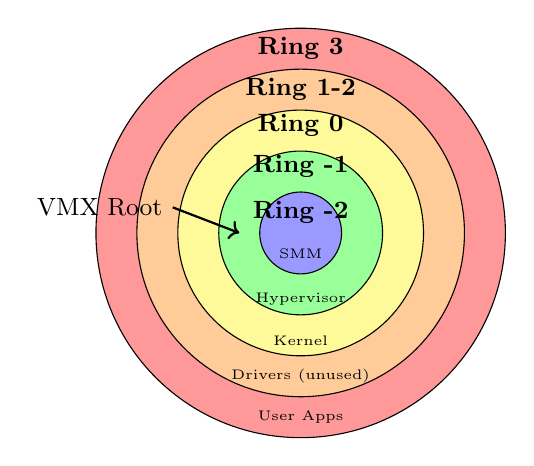
\begin{tikzpicture}[scale=0.65,
                ring num/.style={font=\small\bfseries},
                ring usage/.style={font=\tiny}]
                % Draw visible rings first
                \draw[fill=red!40] (0,0) circle (4cm);
                \draw[fill=orange!40] (0,0) circle (3.2cm);
                \draw[fill=yellow!40] (0,0) circle (2.4cm);

                % Standard rings labels - number at top, usage at bottom
                \node[ring num] at (0,3.6) {Ring 3};
                \node[ring usage] at (0,-3.6) {User Apps};

                \node[ring num] at (0,2.8) {Ring 1-2};
                \node[ring usage] at (0,-2.8) {Drivers (unused)};

                \node[ring num] at (0,2.1) {Ring 0};
                \node[ring usage] at (0,-2.1) {Kernel};

                % Hidden rings revealed on pause
                \onslide<2->{
                    \draw[fill=green!40] (0,0) circle (1.6cm);
                    \node[ring num] at (0,1.3) {Ring -1};
                    \node[ring usage] at (0,-1.3) {Hypervisor};
                    \draw[thick,<-] (-1.2,0) -- (-2.5,0.5) node[left] {\small VMX Root};
                }

                \onslide<3->{
                    \draw[fill=blue!40] (0,0) circle (0.8cm);
                    \node[ring num] at (0,0.4) {Ring -2};
                    \node[ring usage] at (0,-0.4) {SMM};
                }
            \end{tikzpicture}
        \end{column}
    \end{columns}
\end{frame}

\begin{frame}{ARM TrustZone - Trusted Execution Environment (TEE)}
    \begin{center}
        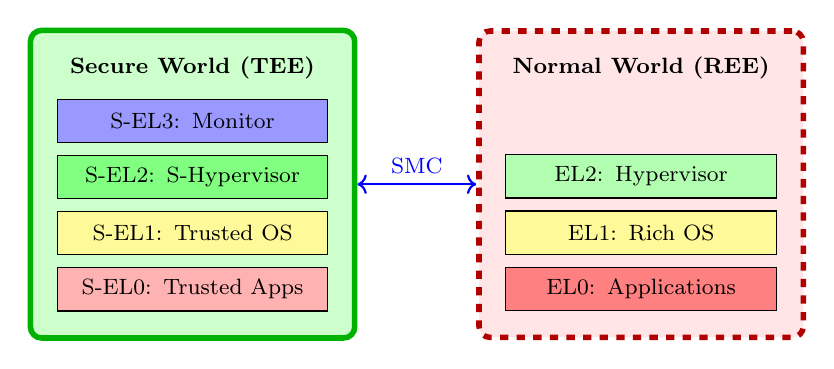
\begin{tikzpicture}[font=\footnotesize,
            level/.style={draw, text width=3.2cm, minimum height=0.55cm, align=center},
            empty/.style={draw=none, text width=3.2cm, minimum height=0.55cm}]

            % Secure World levels as matrix with named label
            \matrix[matrix of nodes, row sep=0.15cm, nodes={level},
                    label={[name=slabel, font=\footnotesize\bfseries]above:Secure World (TEE)}] (secure) {
                |[fill=blue!40]| S-EL3: Monitor \\
                |[fill=green!50]| S-EL2: S-Hypervisor \\
                |[fill=yellow!40]| S-EL1: Trusted OS \\
                |[fill=red!30]| S-EL0: Trusted Apps \\
            };

            % Secure World container using fit (includes label)
            \begin{scope}[on background layer]
                \node[rounded corners, fill=green!20, draw=green!70!black, line width=2pt,
                      fit=(slabel)(secure), inner sep=6pt] (scontainer) {};
            \end{scope}

            % Normal World levels as matrix with phantom top row
            \matrix[matrix of nodes, row sep=0.15cm, nodes={level},
                    right=2cm of secure,
                    label={[name=nlabel, font=\footnotesize\bfseries]above:Normal World (REE)}] (normal) {
                |[empty]| \\
                |[fill=green!30]| EL2: Hypervisor \\
                |[fill=yellow!40]| EL1: Rich OS \\
                |[fill=red!50]| EL0: Applications \\
            };

            % Normal World container using fit (includes label)
            \begin{scope}[on background layer]
                \node[rounded corners, fill=red!10, draw=red!70!black, line width=2pt, dashed,
                      fit=(nlabel)(normal), inner sep=6pt] (ncontainer) {};
            \end{scope}

            % SMC transition
            \draw[<->, thick, blue] (scontainer.east) -- (ncontainer.west) node[midway, above] {SMC};
        \end{tikzpicture}
    \end{center}

    \begin{columns}[T]
        \begin{column}{0.5\textwidth}
            \textbf{TEE Use Cases:}
            \begin{itemize}
                \item DRM content protection
                \item Mobile payments
                \item Biometric authentication
                \item Key management
            \end{itemize}
        \end{column}
        \begin{column}{0.5\textwidth}
            \textbf{TEE = Trusted Execution Environment}
            \begin{itemize}
                \item Isolated from Rich OS (REE)
                \item Secure boot chain
                \item Cryptographic operations
                \item Hardware root of trust
            \end{itemize}
        \end{column}
    \end{columns}
\end{frame}

\begin{frame}{Virtualization Security}
    \begin{columns}
        \begin{column}{0.5\textwidth}
            \textbf{Intel VT-x Features:}
            \begin{itemize}
                \item VMX root/non-root modes
                \item VMCS (VM Control Structure)
                \item EPT (Extended Page Tables)
                \item VPID (Virtual Processor ID)
            \end{itemize}

            \vspace{0.3cm}
            \textbf{VM Exits:}
            \begin{itemize}
                \item Privileged instructions
                \item Page faults
                \item I/O operations
                \item MSR access
            \end{itemize}
        \end{column}
        \begin{column}{0.5\textwidth}
            \begin{tikzpicture}[
                box/.style={draw, thick, minimum width=3.2cm, minimum height=1cm, align=center, font=\small},
                vm/.style={draw, thick, minimum width=1.5cm, minimum height=0.8cm, rounded corners=3pt,
                          align=center, font=\small, text depth=0.3cm},
                guestos/.style={draw, thick, minimum width=1.5cm, minimum height=0.6cm,
                               fill=white, align=center, font=\scriptsize, rounded corners=2pt}]

                % Hardware (bottom layer)
                \node[box, fill=black!20, minimum width=5.2cm] (hw) {\textbf{Hardware}};

                % Hypervisor (Host) - middle layer
                \node[box, fill=orange!30, minimum width=5.2cm, above=0.6cm of hw] (vmm)
                    {\textbf{Hypervisor (Host)}};

                % Guest/Host boundary
                \coordinate (boundary-left) at ([xshift=-2.6cm]vmm.north);
                \coordinate (boundary-right) at ([xshift=2.6cm]vmm.north);

                \draw[very thick, red!70, dashed, line cap=round]
                    (boundary-left) -- (boundary-right)
                    node[pos=0.05, above=2pt, font=\small, text=blue!70, fill=white, inner sep=2pt] {Guest}
                    node[pos=0.95, below=2pt, font=\small, text=red!70, fill=white, inner sep=2pt] {Host};

                % VM containers (top layer)
                \node[vm, fill=blue!30, above left=1.2cm and 0.3cm of vmm.north] (vm1) {\textbf{VM1}};
                \node[vm, fill=green!30, above right=1.2cm and 0.3cm of vmm.north] (vm2) {\textbf{VM2}};

                % Guest OS nodes - anchored to south of VMs
                \node[guestos, below=2mm of vm1.south, anchor=north] (gos1) {Guest OS};
                \node[guestos, below=2mm of vm2.south, anchor=north] (gos2) {Guest OS};

                % EPT connections with organogram icons
                \draw[thick, blue!70!black] (gos1.south) -- (gos1.south |- vmm.north);
                \node[inner sep=0pt] at ($(gos1.south)!0.5!(gos1.south |- vmm.north)$)
                    {\includegraphics[width=0.4cm]{figures/noun-organogram-5851660.png}};

                \draw[thick, blue!70!black] (gos2.south) -- (gos2.south |- vmm.north);
                \node[inner sep=0pt] at ($(gos2.south)!0.5!(gos2.south |- vmm.north)$)
                    {\includegraphics[width=0.4cm]{figures/noun-organogram-5851660.png}};

                % VMM to Hardware connection
                \draw[<->, thick, gray!70] (vmm.south) -- (hw.north);
            \end{tikzpicture}
        \end{column}
    \end{columns}
\end{frame}

\begin{frame}{EPT/NPT - Nested Page Tables}
    \begin{columns}
        \begin{column}{0.5\textwidth}
            \textbf{Problem:}
            \begin{itemize}
                \item Guest OS manages its own page tables
                \item Guest thinks it controls physical memory
                \item Hypervisor must translate guest physical $\rightarrow$ host physical
            \end{itemize}

            \vspace{0.3cm}
            \textbf{Solution: EPT/NPT}
            \begin{itemize}
                \item \textbf{EPT}: Intel's Extended Page Tables
                \item \textbf{NPT}: AMD's Nested Page Tables
                \item Hardware-accelerated 2D page walk
            \end{itemize}

            \vspace{0.3cm}
            \textbf{Address Translation:}
            \begin{enumerate}
                \item Guest Virtual $\rightarrow$ Guest Physical (guest page tables)
                \item Guest Physical $\rightarrow$ Host Physical (EPT/NPT)
            \end{enumerate}
        \end{column}
        \begin{column}{0.5\textwidth}
            \textbf{Performance Impact:}

            \begin{tcolorbox}[colback=yellow!10, title={\small Native (No Virtualization)}]
                {\scriptsize
                \textbf{4-level page walk:}
                \begin{itemize}
                    \item 4 memory accesses
                    \item CR3 $\rightarrow$ PML4 $\rightarrow$ PDP $\rightarrow$ PD $\rightarrow$ PT
                \end{itemize}
                }
            \end{tcolorbox}

            \vspace{0.2cm}
            \begin{tcolorbox}[colback=red!10, title={\small With EPT (Nested)}]
                {\scriptsize
                \textbf{Each guest PTE access needs EPT walk!}
                \begin{itemize}
                    \item Guest walk: 4 accesses
                    \item Each access $\times$ 4 EPT walks
                    \item \textbf{Total: up to $4 \times 5 = 20$ memory accesses}
                \end{itemize}

                \vspace{0.1cm}
                \textbf{Mitigations:}
                \begin{itemize}
                    \item TLB caching (both guest and EPT)
                    \item Large pages (2MB/1GB)
                    \item Typically 2-3$\times$ slowdown
                \end{itemize}
                }
            \end{tcolorbox}
        \end{column}
    \end{columns}
\end{frame}

% Management Engines and IOMMU
\begin{frame}{Intel Management Engine (ME)}
    \begin{columns}
        \begin{column}{0.5\textwidth}
            \textbf{What is Intel ME?}
            \begin{itemize}
                \item Separate processor on Intel chipsets
                \item Runs even when main CPU is off
                \item Has full memory/network access
                \item Runs at Ring -3 privilege
                \item Cannot be disabled on modern systems
            \end{itemize}
            
            \vspace{0.3cm}
            \textbf{Legitimate Uses:}
            \begin{itemize}
                \item Remote management (AMT)
                \item DRM enforcement
                \item Boot verification
                \item Anti-theft features
            \end{itemize}
            
            \vspace{0.3cm}
            \textbf{Security Concerns:}
            \begin{itemize}
                \item Closed source firmware
                \item History of vulnerabilities
                \item Potential backdoor vector
            \end{itemize}
        \end{column}
        \begin{column}{0.5\textwidth}
            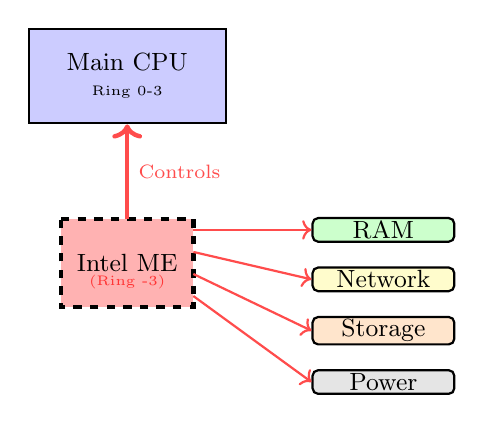
\begin{tikzpicture}[
                resource/.style={draw, thick, minimum width=1.8cm, minimum height=0.3cm,
                               align=center, font=\small, rounded corners=2pt, inner sep=1pt},
                cpu/.style={draw, thick, minimum width=2.5cm, minimum height=1.2cm,
                           fill=blue!20, align=center, font=\small},
                connection/.style={->, thick, red!70}]

                % Intel ME as muxdemux (center-left) - wider and shorter
                \node[muxdemux, muxdemux def={NL=1, NR=4, Rh=2, Lh=2, w=3},
                      fill=red!30, thick, dashed, font=\small, external pins width=0] (me)
                    {Intel ME};

                % Ring privilege level label (clearer)
                \node[font=\tiny, below=1pt of me.center, anchor=north, text=red!80]
                    {(Ring -3)};

                % Main CPU above ME
                \node[cpu, above=1.2cm of me.top] (cpu)
                    {Main CPU\\[-2pt]{\tiny Ring 0-3}};

                % Resources on the right side - RAM moved higher, others stacked below
                \node[resource, fill=green!20, above=1.3cm, right=1.5cm of me.rpin 1] (ram) {RAM};
                \node[resource, fill=yellow!20, below=0.3cm of ram] (network) {Network};
                \node[resource, fill=orange!20, below=0.3cm of network] (storage) {Storage};
                \node[resource, fill=gray!20, below=0.3cm of storage] (power) {Power};

                % ME connections to resources
                \draw[connection] (me.rpin 1) -- (ram.west);
                \draw[connection] (me.rpin 2) -- (network.west);
                \draw[connection] (me.rpin 3) -- (storage.west);
                \draw[connection] (me.rpin 4) -- (power.west);

                % ME controls CPU
                \draw[connection, ultra thick] (me.top) -- (cpu.south)
                    node[midway, right, font=\scriptsize, text=red!70] {Controls};
            \end{tikzpicture}

            \vspace{0.3cm}
            \begin{tcolorbox}[colback=yellow!20]
                \small
                \textbf{Similar Systems:}
                \begin{itemize}
                    \item AMD PSP (Platform Security Processor)
                    \item ARM TrustZone
                \end{itemize}
            \end{tcolorbox}
        \end{column}
    \end{columns}
\end{frame}

\begin{frame}{IOMMU - Input/Output Memory Management Unit}
    \begin{columns}
        \begin{column}{0.55\textwidth}
            \textbf{What is IOMMU?}
            \begin{itemize}
                \item Hardware unit controlling device DMA
                \item Maps device addresses to physical memory
                \item Similar to MMU but for devices
            \end{itemize}

            \vspace{0.3cm}
            \textbf{Key Features:}
            \begin{itemize}
                \item \textbf{PASID:} Process Address Space ID
                \begin{itemize}
                    \item Like ASID but for devices
                    \item Allows device access to specific process memory
                \end{itemize}
                \item \textbf{Protection Granularity:} Page-level (4KB)
                \item \textbf{Interrupt Remapping:} Prevents interrupt injection
            \end{itemize}
        \end{column}
        \begin{column}{0.45\textwidth}
            \centering
            \begin{tikzpicture}[font=\footnotesize, scale=1.3, every node/.style={scale=1.3}]
                % Memory at top right
                \node[inner sep=0pt] (mem)
                    {\includegraphics[width=1cm]{figures/noun-ram-7483151.png}};
                \node[font=\tiny, above=1pt of mem] {Memory};

                % MMU as simple rectangle, left of Memory
                \node[draw, thick, fill=blue!20, minimum width=1.2cm, minimum height=0.6cm,
                      font=\scriptsize, left=0.4cm of mem] (mmu) {MMU};

                % CPU image left of MMU
                \node[inner sep=0pt, left=0.4cm of mmu] (cpu)
                    {\includegraphics[width=1cm]{figures/noun-cpu-8157304.png}};
                \node[font=\tiny, above=1pt of cpu] {CPU};

                % Wire CPU to MMU to Memory
                \draw[->, thick, blue] (cpu.east) -- (mmu.west);
                \draw[->, thick, blue] (mmu.east) -- (mem.west);

                % IOMMU as muxdemux - below MMU, with 3 bottom pins
                \node[muxdemux, muxdemux def={NB=3, Rh=1.5, Lh=1.5, w=3},
                      fill=yellow!30, thick, font=\small,
                      external pins width=0, below=0.8cm of mmu] (iommu) {IOMMU};

                % Wire from IOMMU top to Memory (with label on right)
                \draw[->, thick, green!60!black] (iommu.top) -- ++(0,0.15) -| (mem.south)
                    node[pos=0.75, right, font=\scriptsize] {Allowed};

                % Device images at bottom - spread out with explicit x offsets
                \node[inner sep=0pt, below=0.5cm of iommu.bpin 2] (nic)
                    {\includegraphics[width=0.8cm]{figures/noun-network-card-7443121.png}};
                \node[font=\tiny, below=1pt of nic] {NIC};

                \node[inner sep=0pt, left=0.8cm of nic] (usb)
                    {\includegraphics[width=0.8cm]{figures/noun-usb-8182582.png}};
                \node[font=\tiny, below=1pt of usb] {USB};

                \node[inner sep=0pt, right=0.8cm of nic] (gpu)
                    {\includegraphics[width=0.8cm]{figures/noun-graphics-card-1036913.png}};
                \node[font=\tiny, below=1pt of gpu] {GPU};

                % Device connections to IOMMU (DMA requests)
                \draw[->, thick, red] (usb.north) -- ++(0,0.15) -| (iommu.bpin 1);
                \draw[->, thick, red] (nic.north) -- (iommu.bpin 2);
                \draw[->, thick, red] (gpu.north) -- ++(0,0.15) -| (iommu.bpin 3);

                % Blocked indicator with X image
                \node[inner sep=0pt, right=0.6cm of iommu.right] (blocked)
                    {\includegraphics[width=0.5cm]{figures/noun-x-2222229.png}};
                \node[red, font=\scriptsize, below=1pt of blocked] {Blocked};

                % Show a blocked path attempt
                \draw[->, thick, red, dashed] (iommu.right) -- (blocked.west);
            \end{tikzpicture}
        \end{column}
    \end{columns}
\end{frame}

\begin{frame}{IOMMU - Attack Prevention}
    \begin{columns}
        \begin{column}{0.5\textwidth}
            \textbf{CPU-Initiated Attacks:}
            \begin{itemize}
                \item Compromised driver attempts DMA
                \item Kernel bug triggers bad DMA request
                \item IOMMU validates all translations
            \end{itemize}

            \vspace{0.5cm}
            \textbf{Device-Initiated Attacks:}
            \begin{itemize}
                \item Malicious firmware in peripherals
                \item Compromised network cards
                \item Rogue Thunderbolt devices
                \item USB devices with DMA capability
            \end{itemize}
        \end{column}
        \begin{column}{0.5\textwidth}
            \textbf{Attacks Prevented:}
            \begin{itemize}
                \item \textcolor{red}{DMA attacks} (BadUSB, Thunderstrike)
                \item \textcolor{red}{Malicious devices} reading memory
                \item \textcolor{red}{Driver bugs} corrupting memory
            \end{itemize}

            \vspace{0.5cm}
            \begin{tcolorbox}[colback=yellow!20]
                \textbf{Limitation:} Protection is page-granular (4KB). If two data structures share a page, device can access both!
            \end{tcolorbox}
        \end{column}
    \end{columns}
\end{frame}

\begin{frame}{IOMMU - Shared Buffer Problem}
    \begin{columns}
        \begin{column}{0.5\textwidth}
            \textbf{The Problem:}
            \begin{itemize}
                \item IOMMU protection is page-granular
                \item Device needs access to buffer A
                \item Buffer B is on same 4KB page
                \item Device can access both!
            \end{itemize}

            \vspace{-5mm}
            \begin{tcolorbox}[colback=blue!20]
                \textbf{Solutions:}
                \begin{itemize}
                    \item Align DMA buffers to page boundaries
                    \item Use bounce buffers (copy to isolated page)
                    \item Sub-page protection (future hardware)
                \end{itemize}
            \end{tcolorbox}
        \end{column}
        \begin{column}{0.5\textwidth}
            \begin{tikzpicture}[font=\footnotesize, scale=1.3, every node/.style={scale=1.3},
                buffer/.style={draw, minimum width=2cm, minimum height=0.8cm, align=center}]
                % Memory page container
                \node[draw, fill=gray!10, minimum width=5cm, minimum height=1.8cm] (page) {};
                \node[font=\small\bfseries, above=0pt of page.north, anchor=south] {4KB Page};

                % Buffers inside page
                \node[buffer, fill=green!30, left=0.2cm of page.center, anchor=east] (bufA)
                    {Buffer A\\[-2pt]{\tiny (Intended)}};
                \node[buffer, fill=red!30, right=0.2cm of page.center, anchor=west] (bufB)
                    {Buffer B\\[-2pt]{\tiny (Sensitive)}};

                % IOMMU below page with NT=2, NB=2
                \node[muxdemux, muxdemux def={NT=2, NB=2, Rh=1.2, Lh=1.2, w=2.5},
                      fill=yellow!30, thick, font=\scriptsize,
                      external pins width=0, below=1cm of page] (iommu) {IOMMU};

                % Device icon below IOMMU
                \node[inner sep=0pt, below=0.6cm of iommu] (dev)
                    {\includegraphics[width=0.8cm]{figures/noun-network-card-7443121.png}};
                \node[font=\tiny, below=1pt of dev] {Device};

                % Device to IOMMU - two transactions
                \draw[->, thick, green!60!black] (dev.north) -- ++(0,0.2) -| (iommu.bpin 1);
                \draw[->, thick, red, dashed] (dev.north) -- ++(0,0.1) -| (iommu.bpin 2);

                % IOMMU to Buffer A (intended)
                \draw[->, thick, green!60!black] (iommu.tpin 1) -- (bufA.south)
                    node[midway, left, font=\tiny] {Allowed};

                % IOMMU to Buffer B (unintended leak)
                \draw[->, thick, red, dashed] (iommu.tpin 2) -- (bufB.south)
                    node[midway, right, font=\tiny, text=red] {Leaks!};
            \end{tikzpicture}
        \end{column}
    \end{columns}
\end{frame}

% Section 4: Trusted Execution
\section{Trusted Execution Environments}

\begin{frame}{Why Trusted Execution Environments (TEEs)?}
    \begin{columns}[T]
        \begin{column}{0.5\textwidth}
            \textbf{The Problem:}
            \begin{itemize}
                \item Cloud computing $\rightarrow$ running on untrusted infrastructure
                \item Cloud provider has physical access
                \item Hypervisor has full control over VMs
                \item Can read memory, modify code, inject malware
            \end{itemize}

            \vspace{0.3cm}
            \textbf{Trust Boundary Shift:}
            \begin{itemize}
                \item Traditional: Trust the cloud provider
                \item TEE: Trust only the hardware/CPU
                \item Provider is explicitly \textcolor{red}{untrusted}
            \end{itemize}
        \end{column}
        \begin{column}{0.5\textwidth}
            \textbf{Use Cases:}
            \begin{itemize}
                \item Confidential computing in public cloud
                \item Processing sensitive data (medical, financial)
                \item Multi-party computation
                \item Secure enclaves for ML models
            \end{itemize}

            \vspace{0.3cm}
            \begin{tcolorbox}[colback=blue!10, title={\small Goal}]
                \textbf{Run code on someone else's hardware without them being able to:}%
                \begin{itemize}
                    \item Read your data
                    \item Modify your code
                    \item Tamper with execution
                \end{itemize}
                Even with physical access!
            \end{tcolorbox}

            \vspace{0.2cm}
            {\small \textit{Different targets:}
            \begin{itemize}
                \item \textbf{Intel TDX/AMD SEV}: Full VM isolation
                \item \textbf{Intel SGX/ARM TrustZone}: Process-level isolation
            \end{itemize}
            }
        \end{column}
    \end{columns}
\end{frame}

\begin{frame}{TEE Requirements - How Do We Achieve This?}
    \begin{columns}
        \begin{column}{0.5\textwidth}
            \textbf{1. Memory Encryption:}
            \begin{itemize}
                \item Encrypt all TEE memory
                \item Each TEE has unique encryption key
                \item Hardware encrypts/decrypts transparently
                \item Prevents physical memory dumps
            \end{itemize}

            \vspace{0.3cm}
            \textbf{2. Hardware-Enforced Isolation:}
            \begin{itemize}
                \item CPU enforces access control
                \item Hypervisor \textcolor{red}{cannot} access TEE memory
                \item DMA attacks blocked (IOMMU protection)
                \item Hardware prevents tampering
            \end{itemize}
        \end{column}
        \begin{column}{0.5\textwidth}
            \textbf{3. Remote Attestation:}
            \begin{itemize}
                \item Prove you're running in genuine TEE
                \item Relies on secure boot chain
                \item CPU signs measurement report
                \item Client verifies before sending secrets
            \end{itemize}

            \vspace{0.2cm}
            \begin{tcolorbox}[colback=green!10, title={\small Attestation Flow}]
                {\scriptsize
                \textbf{1.} TEE measures code/data (hash)\\
                \textbf{2.} CPU signs measurement with private key\\
                \textbf{3.} Client verifies signature with CPU's public key\\
                \textbf{4.} If valid $\rightarrow$ client sends encrypted secrets\\
                \vspace{0.1cm}

                \textit{Relies on:}
                \begin{itemize}
                    \item Secure boot (chain of trust)
                    \item Hardware root of trust (TPM/fused keys)
                    \item CPU manufacturer's PKI
                \end{itemize}
                }
            \end{tcolorbox}
        \end{column}
    \end{columns}
\end{frame}

\begin{frame}{TEE Memory Protection Approaches}
    \begin{columns}[T]
        \begin{column}{0.5\textwidth}
            \textbf{1. Access Control Based:}
            \begin{itemize}
                \item CPU enforces access restrictions
                \item Hypervisor/OS \textcolor{red}{blocked} from accessing TEE memory
                \item Page table attributes control access
                \item Fast (no encryption overhead)
            \end{itemize}

            \vspace{0.2cm}
            {\small \textbf{Examples:}
            \begin{itemize}
                \item Intel SGX: EPCM (Enclave Page Cache Map)
                \item ARM TrustZone: NS bit (secure/non-secure)
            \end{itemize}
            }

            \vspace{0.2cm}
            {\small \textcolor{red}{\textbf{Limitation:}} Vulnerable to physical attacks (cold boot, bus snooping)}

            \vspace{0.3cm}
            \textbf{2. Encryption Based:}
            \begin{itemize}
                \item Memory encrypted in DRAM
                \item Each TEE has unique key
                \item Hardware encrypts/decrypts on memory bus
                \item Protects against physical attacks
            \end{itemize}

            \vspace{0.2cm}
            {\small \textbf{Examples:}
            \begin{itemize}
                \item AMD SEV: Per-VM encryption keys
                \item Intel MKTME: Multi-key total memory encryption
            \end{itemize}
            }
        \end{column}
        \begin{column}{0.5\textwidth}
            \textbf{3. Hybrid Approaches:}

            \vspace{0.2cm}
            Combine both for defense in depth:
            \begin{itemize}
                \item Access control prevents software attacks
                \item Encryption prevents physical attacks
            \end{itemize}

            \vspace{0.2cm}
            {\small \textbf{Examples:}
            \begin{itemize}
                \item AMD SEV-SNP: Encryption + RMP (Reverse Map Table)
                \item Intel TDX: Encryption + SEPT (Secure EPT)
            \end{itemize}
            }

            \vspace{0.3cm}
            \begin{tcolorbox}[colback=blue!10, title={\small Memory Protection Trade-offs}]
                {\scriptsize
                \textbf{Access Control Only:}
                \begin{itemize}
                    \item $\checkmark$ Fast, no encryption overhead
                    \item $\times$ Physical attacks possible
                \end{itemize}

                \vspace{0.1cm}
                \textbf{Encryption Only:}
                \begin{itemize}
                    \item $\checkmark$ Protects against physical attacks
                    \item $\times$ Performance overhead (5-15\%)
                    \item $\times$ Complex key management
                \end{itemize}

                \vspace{0.1cm}
                \textbf{Hybrid:}
                \begin{itemize}
                    \item $\checkmark$ Defense in depth
                    \item $\times$ Complexity + overhead
                \end{itemize}
                }
            \end{tcolorbox}
        \end{column}
    \end{columns}
\end{frame}

\begin{frame}{Secure VMs vs Secure Enclaves}
    \begin{columns}[T]
        \begin{column}{0.5\textwidth}
            \textbf{Secure Enclaves (Process-Level):}

            \vspace{0.2cm}
            \textbf{Concept:}
            \begin{itemize}
                \item Isolate parts of an application
                \item Trust boundary \textit{within} a VM/OS
                \item Small trusted computing base (TCB)
                \item Application explicitly uses enclave
            \end{itemize}

            \vspace{0.2cm}
            \textbf{Threat Model:}
            \begin{itemize}
                \item Untrusted OS/kernel
                \item Untrusted applications
                \item Privileged software is adversary
            \end{itemize}

            \vspace{0.2cm}
            \textbf{Examples:}
            \begin{itemize}
                \item \textbf{Intel SGX}: x86 enclave instructions
                \item \textbf{ARM TrustZone}: Secure/Normal worlds
                \item \textbf{AMD SEV-ES}: Single VM encryption
            \end{itemize}

            \vspace{0.2cm}
            \textbf{Use Cases:}
            \begin{itemize}
                \item Protect cryptographic keys
                \item Secure password verification
                \item DRM (Digital Rights Management)
                \item Biometric authentication
            \end{itemize}
        \end{column}
        \begin{column}{0.5\textwidth}
            \textbf{Secure VMs (VM-Level):}

            \vspace{0.2cm}
            \textbf{Concept:}
            \begin{itemize}
                \item Isolate entire virtual machines
                \item Trust boundary at hypervisor level
                \item Large TCB (entire VM)
                \item Transparent to guest OS
            \end{itemize}

            \vspace{0.2cm}
            \textbf{Threat Model:}
            \begin{itemize}
                \item Untrusted hypervisor
                \item Untrusted cloud provider
                \item Physical access attacks
            \end{itemize}

            \vspace{0.2cm}
            \textbf{Examples:}
            \begin{itemize}
                \item \textbf{Intel TDX}: Trust Domain Extensions
                \item \textbf{AMD SEV-SNP}: Secure Nested Paging
                \item \textbf{ARM CCA}: Confidential Compute Architecture
            \end{itemize}

            \vspace{0.2cm}
            \textbf{Use Cases:}
            \begin{itemize}
                \item Confidential computing in public cloud
                \item Lift-and-shift existing workloads
                \item Multi-tenant isolation
                \item Regulatory compliance (GDPR, HIPAA)
            \end{itemize}

            \vspace{0.2cm}
            \begin{tcolorbox}[colback=green!10]
                {\scriptsize \textbf{Key Difference:}\\
                Enclaves require application changes.\\
                Secure VMs work with unmodified OS.}
            \end{tcolorbox}
        \end{column}
    \end{columns}
\end{frame}

\begin{frame}{Intel TDX (Trust Domain Extensions)}
    \begin{columns}
        \begin{column}{0.5\textwidth}
            \textbf{Who Protects Whom:}
            \begin{itemize}
                \item \textcolor{green!70!black}{\textbf{Protected:}} Guest VMs
                \item \textcolor{red}{\textbf{Threat:}} Cloud Provider
                \item \textcolor{blue}{\textbf{Enforcer:}} CPU Hardware
            \end{itemize}
            
            \vspace{0.3cm}
            \textbf{Protection Guarantees:}
            \begin{itemize}
                \item Confidentiality from hypervisor
                \item Memory encryption per VM
                \item CPU-attested execution
                \item Secure EPT (S-EPT)
            \end{itemize}
            
            \vspace{0.3cm}
            \textbf{Use Case:}
            \begin{tcolorbox}[colback=green!10]
                \small
                Run sensitive workloads on untrusted cloud infrastructure
            \end{tcolorbox}
        \end{column}
        \begin{column}{0.5\textwidth}
            \begin{tikzpicture}[scale=0.7, font=\small,
                threat/.style={draw, fill=red!30, minimum width=3cm, minimum height=0.6cm, font=\small\bfseries},
                vm/.style={draw, line width=1pt, minimum width=1.5cm, minimum height=1.5cm, align=center},
                cpu/.style={draw, fill=yellow!30, minimum width=4.8cm, minimum height=0.8cm, font=\small\bfseries},
                barrier/.style={ultra thick, blue}]

                % CPU enforcement (top)
                \node[cpu] (cpu) {CPU (TDX Module)};

                % Protected VMs
                \node[vm, fill=green!30, draw=green!70!black, below left=0.5cm of cpu.south] (vm1) {
                    \textbf{VM1}\\[-2pt]{\tiny Customer A}};
                \node[vm, fill=blue!30, draw=blue!70!black, below right=0.5cm of cpu.south] (vm2) {
                    \textbf{VM2}\\[-2pt]{\tiny Customer B}};

                % Protection barrier
                \draw[barrier] ([xshift=-0.5cm]vm1.south west) -- ([xshift=0.5cm]vm2.south east)
                    node[right, font=\small] {TDX};

                % Threat Actor (bottom)
                \node[inner sep=0pt, below=2cm of cpu] (provider)
                    {\includegraphics[width=1.5cm]{figures/noun-cloud-5095064.png}};
                \node[font=\tiny, below=1pt of provider] {Cloud Provider (Untrusted)};

                % Attack attempts with X marks
                \draw[->, thick, red] (provider.north) -- ++(0,0.8)
                    node[midway, right, font=\tiny] {Read};
                \draw[->, thick, red] ([xshift=-0.8cm]provider.north) -- ++(0,0.8)
                    node[midway, left, font=\tiny] {Modify};

                % X marks for blocked attacks
                \node[inner sep=0pt] at ([yshift=0.5cm]provider.north)
                    {\includegraphics[width=0.4cm]{figures/noun-x-2222229.png}};
                \node[inner sep=0pt] at ([xshift=-0.8cm, yshift=0.5cm]provider.north)
                    {\includegraphics[width=0.4cm]{figures/noun-x-2222229.png}};

                % Protection arrows from CPU
                \draw[->, thick, green!60!black] (cpu.south) -- (vm1.north);
                \draw[->, thick, green!60!black] (cpu.south) -- (vm2.north);
            \end{tikzpicture}
        \end{column}
    \end{columns}
\end{frame}

\begin{frame}{AMD SEV-SNP - Secure Encrypted Virtualization}
    \begin{columns}
        \begin{column}{0.5\textwidth}
            \textbf{What SEV-SNP Protects Against:}
            \begin{itemize}
                \item \textcolor{red}{Malicious hypervisor}
                \item \textcolor{red}{Physical memory attacks}
                \item \textcolor{red}{VM memory inspection}
                \item \textcolor{red}{Replay attacks}
            \end{itemize}
            
            \vspace{0.3cm}
            \textbf{Key Features:}
            \begin{itemize}
                \item \textbf{SEV:} Memory encryption per-VM
                \item \textbf{SEV-ES:} Register state encryption
                \item \textbf{SEV-SNP:} Integrity protection
            \end{itemize}
            
            \vspace{0.3cm}
            \textbf{SNP Additions:}
            \begin{itemize}
                \item Reverse Map Table (RMP)
                \item Page ownership tracking
                \item Prevents remapping attacks
                \item Guest-controlled page validation
            \end{itemize}
        \end{column}
        \begin{column}{0.5\textwidth}
            \begin{tikzpicture}[
                vm/.style={draw, thick, minimum width=2.2cm, minimum height=1.8cm,
                          align=center, font=\small, rounded corners=2pt},
                amd sp/.style={draw, thick, fill=yellow!30, minimum width=3.5cm,
                              minimum height=0.8cm, align=center, font=\small, inner sep=2pt},
                connection/.style={<->, thick},
                attack/.style={->, thick, red, dashed}]

                % AMD Security Processor at top
                \node[amd sp] (amdsp) {\textbf{AMD SP}};

                % Protected VMs below AMD SP
                \node[vm, fill=green!30, below left=1cm and 0.3cm of amdsp.south] (vm1)
                    {\textbf{VM1}\\[-2pt]\small Encrypted\\[-2pt]{\tiny Key1}};
                \node[vm, fill=blue!30, below right=1cm and 0.3cm of amdsp.south] (vm2)
                    {\textbf{VM2}\\[-2pt]\small Encrypted\\[-2pt]{\tiny Key2}};

                % Protection connections
                \draw[connection, green!70!black] (vm1.north) -- (amdsp.south);
                \draw[connection, blue!70!black] (vm2.north) -- (amdsp.south);

                % Untrusted Cloud Provider at bottom
                \node[inner sep=0pt, below=2cm of amdsp.south] (cloud)
                    {\includegraphics[width=1.8cm]{figures/noun-cloud-5095064.png}};
                \node[font=\tiny, below=1pt of cloud] {Cloud Provider (Untrusted)};

                % Blocked attack attempts with X marks
                \draw[attack] (cloud.north) -- ++(0, 0.6cm);
                \node[inner sep=0pt] at ([yshift=3mm]cloud.north)
                    {\includegraphics[width=0.4cm]{figures/noun-x-2222229.png}};

                \draw[attack] ([xshift=-8mm]cloud.north) -- ++(0, 0.6cm);
                \node[inner sep=0pt] at ([xshift=-8mm, yshift=3mm]cloud.north)
                    {\includegraphics[width=0.4cm]{figures/noun-x-2222229.png}};

                % Attack labels
                \node[red, font=\tiny, left] at ([xshift=-8mm, yshift=3mm]cloud.north) {Read};
                \node[red, font=\tiny, right] at ([xshift=8mm, yshift=3mm]cloud.north) {Modify};
            \end{tikzpicture}

            \vspace{0.3cm}
            \begin{tcolorbox}[colback=yellow!20]
                \textbf{RMP (Reverse Map Table):}
                \begin{itemize}
                    \item Tracks page ownership (ASID)
                    \item Validates page access
                    \item Hardware-enforced
                \end{itemize}
            \end{tcolorbox}
        \end{column}
    \end{columns}
\end{frame}

\begin{frame}[fragile]{Merkle Trees for Memory Freshness}
    \begin{columns}
        \begin{column}{0.5\textwidth}
            \textbf{The Replay Problem:}
            \begin{itemize}
                \item Encryption prevents reading
                \item But not replay attacks
                \item Attacker saves old ciphertext
                \item Replays it later
            \end{itemize}
            
            \vspace{0.3cm}
            \textbf{Merkle Tree Solution:}
            \begin{itemize}
                \item Tree of cryptographic hashes
                \item Root stored in secure location
                \item Each node hashes its children
                \item Detects any modification
            \end{itemize}
            
            \vspace{0.3cm}
            \textbf{Intel SGX Implementation:}
            \begin{itemize}
                \item 8-ary tree (8 children per node)
                \item Counters at leaf level
                \item MAC for each cache line
                \item Root in on-chip SRAM
            \end{itemize}
        \end{column}
        \begin{column}{0.5\textwidth}
            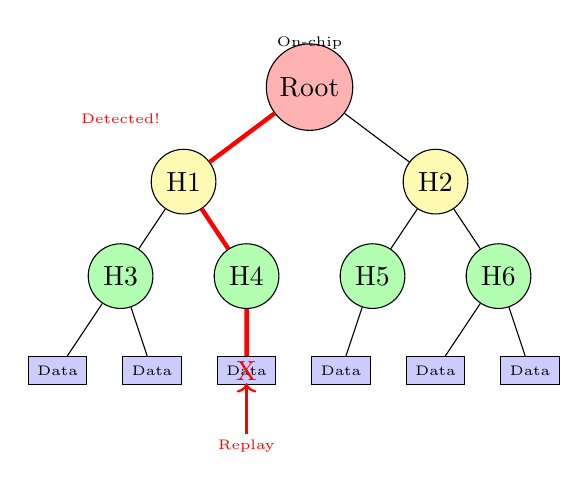
\begin{tikzpicture}[scale=0.8]
                % Root
                \node[draw,fill=red!30,circle] (root) at (4,5) {Root};
                \node at (4,5.7) {\tiny On-chip};
                
                % Level 1
                \node[draw,fill=yellow!30,circle] (n1) at (2,3.5) {H1};
                \node[draw,fill=yellow!30,circle] (n2) at (6,3.5) {H2};
                
                % Level 2
                \node[draw,fill=green!30,circle] (n3) at (1,2) {H3};
                \node[draw,fill=green!30,circle] (n4) at (3,2) {H4};
                \node[draw,fill=green!30,circle] (n5) at (5,2) {H5};
                \node[draw,fill=green!30,circle] (n6) at (7,2) {H6};
                
                % Data blocks
                \node[draw,fill=blue!20] (d1) at (0,0.5) {\tiny Data};
                \node[draw,fill=blue!20] (d2) at (1.5,0.5) {\tiny Data};
                \node[draw,fill=blue!20] (d3) at (3,0.5) {\tiny Data};
                \node[draw,fill=blue!20] (d4) at (4.5,0.5) {\tiny Data};
                \node[draw,fill=blue!20] (d5) at (6,0.5) {\tiny Data};
                \node[draw,fill=blue!20] (d6) at (7.5,0.5) {\tiny Data};
                
                % Edges
                \draw[-] (root) -- (n1);
                \draw[-] (root) -- (n2);
                \draw[-] (n1) -- (n3);
                \draw[-] (n1) -- (n4);
                \draw[-] (n2) -- (n5);
                \draw[-] (n2) -- (n6);
                \draw[-] (n3) -- (d1);
                \draw[-] (n3) -- (d2);
                \draw[-] (n4) -- (d3);
                \draw[-] (n5) -- (d4);
                \draw[-] (n6) -- (d5);
                \draw[-] (n6) -- (d6);
                
                % Attack
                \node[red] at (d3) {X};
                \draw[->,thick,red] (3,-0.5) -- (3,0.3);
                \node[red] at (3,-0.7) {\tiny Replay};
                
                % Detection path
                \draw[ultra thick,red] (d3) -- (n4);
                \draw[ultra thick,red] (n4) -- (n1);
                \draw[ultra thick,red] (n1) -- (root);
                \node[red] at (1,4.5) {\tiny Detected!};
            \end{tikzpicture}
            
            \vspace{0.3cm}
            \begin{tcolorbox}[colback=green!10]
                \small
                \textbf{Freshness Guarantee:}
\begin{minted}[fontsize=\scriptsize]{text}
On Write:
  1. Update data
  2. Update counter
  3. Recalculate hashes to root

On Read:
  1. Verify path to root
  2. Check counter matches
\end{minted}
            \end{tcolorbox}
        \end{column}
    \end{columns}
\end{frame}

\begin{frame}{Intel SGX Enclaves}
    \begin{columns}
        \begin{column}{0.5\textwidth}
            \textbf{SGX - Another TEE Implementation:}
            \begin{itemize}
                \item Isolated execution environment (TEE)
                \item Encrypted memory (MEE)
                \item Remote attestation
                \item Sealed storage
                \item x86-specific (vs ARM TrustZone)
            \end{itemize}
            
            \vspace{0.3cm}
            \textbf{Instructions:}
            \begin{itemize}
                \item \texttt{ECREATE}: Create enclave
                \item \texttt{EENTER}: Enter enclave
                \item \texttt{EEXIT}: Exit enclave
                \item \texttt{ERESUME}: Resume after AEX
            \end{itemize}
        \end{column}
        \begin{column}{0.5\textwidth}
            \begin{tikzpicture}[
                app/.style={draw, thick, minimum width=5cm, minimum height=4.5cm,
                           fill=gray!15, rounded corners=3pt},
                enclave/.style={draw, very thick, minimum width=3.5cm, minimum height=2.5cm,
                              fill=green!30, rounded corners=3pt, align=center}]

                % Application container
                \node[app] (app) {};
                \node[font=\small\bfseries, below=2pt of app.north] {Application};

                % SGX Enclave - protected region
                \node[enclave] (enclave) at (app.center)
                    {\textbf{SGX Enclave}\\[-2pt]
                     \small Trusted Code\\[-2pt]
                     \small Encrypted Data\\[2pt]
                     \includegraphics[width=0.4cm]{figures/noun-lock-locked-4020631.png}};

                % Untrusted code region
                \node[font=\small, above=2pt of app.south] {Untrusted Code};

                % EPC Memory connection
                \draw[<-, thick, blue!70] (enclave.east) -- ++(1.5cm, 0)
                    node[right, font=\small] {EPC Memory};
            \end{tikzpicture}

            \vspace{0.3cm}
            \textbf{Page Types:} REG, TCS, SECS, VA
        \end{column}
    \end{columns}
\end{frame}

\begin{frame}{MKTME (Multi-Key Total Memory Encryption)}
    \begin{columns}
        \begin{column}{0.5\textwidth}
            \textbf{Features:}
            \begin{itemize}
                \item Multiple encryption keys
                \item Per-VM/container isolation
                \item KeyID in physical address bits
                \item AES-XTS encryption
            \end{itemize}
            
            \vspace{0.3cm}
            \textbf{Key Management:}
            \begin{itemize}
                \item Up to 15 keys (4-bit KeyID)
                \item Software-managed keys
                \item PCONFIG instruction
                \item Key rotation support
            \end{itemize}
        \end{column}
        \begin{column}{0.5\textwidth}
            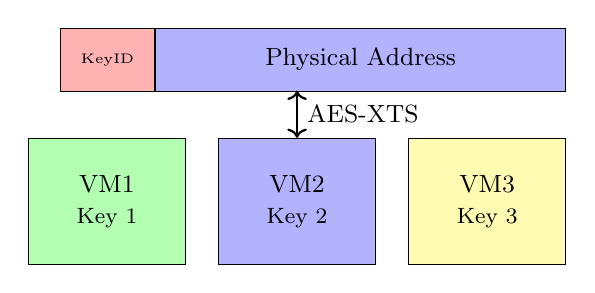
\begin{tikzpicture}[scale=0.6, font=\small,
                addr field/.style={draw, minimum height=0.8cm, anchor=west},
                vm box/.style={draw, minimum width=2cm, minimum height=1.6cm, align=center}]

                % Physical address bar
                \node[addr field, fill=red!30, minimum width=1.2cm] (keyid) at (0,4) {};
                \node[font=\tiny] at (keyid.center) {KeyID};
                \node[addr field, fill=blue!30, minimum width=5.2cm, right=0pt of keyid] (paddr) {};
                \node at (paddr.center) {Physical Address};

                % Memory regions
                \node[vm box, fill=green!30] (vm1) at (1,1) {VM1\\{\footnotesize Key 1}};
                \node[vm box, fill=blue!30, right=0.4cm of vm1] (vm2) {VM2\\{\footnotesize Key 2}};
                \node[vm box, fill=yellow!30, right=0.4cm of vm2] (vm3) {VM3\\{\footnotesize Key 3}};

                % Encryption engine
                \draw[thick,<->] (vm2.north) -- ++(0,1) node[right, midway] {AES-XTS};
            \end{tikzpicture}
            
            \vspace{0.3cm}
            \textbf{Use Cases:}
            \begin{itemize}
                \item Cloud multi-tenancy
                \item Container isolation
                \item Key-based memory domains
            \end{itemize}
        \end{column}
    \end{columns}
\end{frame}

% Section 5: Boot Security
\section{Boot Security}

\begin{frame}{Secure Boot - Implementing Chain of Trust}
    \begin{columns}[T]
        \begin{column}{0.45\textwidth}
            \textbf{Chain of Trust Implementation:}
            \begin{itemize}
                \item Each stage verifies the next
                \item Cryptographic signatures (UEFI)
                \item Hash measurements (TPM)
                \item Extends from boot to runtime
            \end{itemize}

            \vspace{0.2cm}
            \textbf{UEFI Keys:}
            \begin{itemize}
                \item \textbf{PK}: Platform Key (OEM)
                \item \textbf{KEK}: Key Exchange Key
                \item \textbf{db}: Signature Database
                \item \textbf{dbx}: Revoked Signatures
            \end{itemize}

            \vspace{0.2cm}
            \textbf{TPM Role:}
            \begin{itemize}
                \item Stores measurements in PCRs
                \item PCR0-7: Firmware/Boot
                \item PCR8-15: OS/Runtime
                \item Enables remote attestation
            \end{itemize}

            \vspace{0.2cm}
            {\small \textbf{IMA (Integrity Measurement Architecture):}
            \begin{itemize}
                \item Linux kernel subsystem
                \item Measures files before execution
                \item Extends PCR10
                \item Runtime integrity verification
            \end{itemize}
            }
        \end{column}
        \begin{column}{0.55\textwidth}
            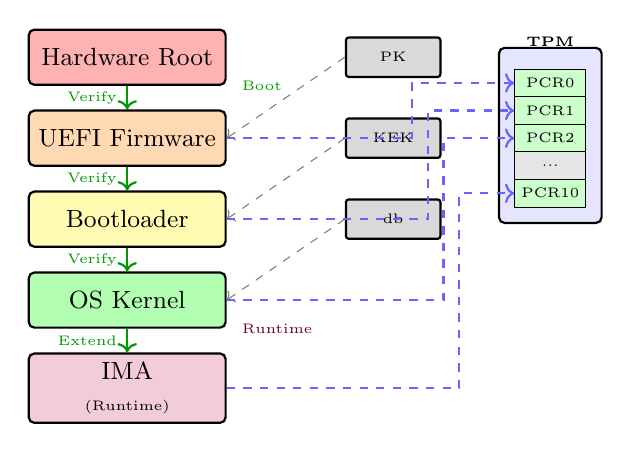
\begin{tikzpicture}[
                chainlink/.style={draw, thick, minimum width=2.5cm, minimum height=0.7cm,
                                 align=center, font=\small, rounded corners=2pt},
                key/.style={draw, thick, minimum width=1.2cm, minimum height=0.5cm,
                           align=center, font=\tiny, fill=gray!30, rounded corners=1pt},
                verify/.style={->, thick, green!60!black},
                measure/.style={->, thick, blue!60, dashed}]

                % Boot Chain - left side
                \node[chainlink, fill=red!30] (hw) {Hardware Root};
                \node[chainlink, fill=orange!30, below=0.3cm of hw] (uefi) {UEFI Firmware};
                \node[chainlink, fill=yellow!30, below=0.3cm of uefi] (bootloader) {Bootloader};
                \node[chainlink, fill=green!30, below=0.3cm of bootloader] (kernel) {OS Kernel};
                \node[chainlink, fill=purple!20, below=0.3cm of kernel] (ima) {IMA\\{\tiny (Runtime)}};

                % Keys - right side
                \node[key, right=1.5cm of hw] (pk) {PK};
                \node[key, right=1.5cm of uefi] (kek) {KEK};
                \node[key, right=1.5cm of bootloader] (db) {db};

                % TPM with PCR matrix - far right
                \matrix[matrix of nodes,
                    nodes={draw, minimum width=0.9cm, minimum height=0.35cm,
                           font=\tiny, fill=green!20, inner sep=1pt},
                    row sep=-\pgflinewidth,
                    right=0.8cm of kek] (pcrs) {
                    PCR0 \\
                    PCR1 \\
                    PCR2 \\
                    |[fill=gray!20]| ... \\
                    PCR10 \\
                };

                % TPM container around PCRs
                \node[font=\tiny\bfseries, above=1pt of pcrs] {TPM};
                \begin{scope}[on background layer]
                    \node[draw, thick, fill=blue!10, rounded corners=2pt,
                          fit={(pcrs) ([yshift=2pt]pcrs.north)}, inner sep=2pt] (tpm) {};
                \end{scope}

                % Verification arrows (green)
                \draw[verify] (hw.south) -- (uefi.north) node[midway, left, font=\tiny] {Verify};
                \draw[verify] (uefi.south) -- (bootloader.north) node[midway, left, font=\tiny] {Verify};
                \draw[verify] (bootloader.south) -- (kernel.north) node[midway, left, font=\tiny] {Verify};
                \draw[verify] (kernel.south) -- (ima.north) node[midway, left, font=\tiny] {Extend};

                % Key usage (dashed to chain)
                \draw[dashed, ->, gray] (pk.west) -- (uefi.east);
                \draw[dashed, ->, gray] (kek.west) -- (bootloader.east);
                \draw[dashed, ->, gray] (db.west) -- (kernel.east);

                % TPM measurement arrows (blue dashed) to specific PCRs - staircase routing
                \draw[measure] (uefi.east) -| ([xshift=-13mm]pcrs-1-1.west) -- (pcrs-1-1.west);
                \draw[measure] (bootloader.east) -| ([xshift=-11mm]pcrs-2-1.west) -- (pcrs-2-1.west);
                \draw[measure] (kernel.east) -| ([xshift=-9mm]pcrs-3-1.west) -- (pcrs-3-1.west);
                \draw[measure] (ima.east) -| ([xshift=-7mm]pcrs-5-1.west) -- (pcrs-5-1.west);

                % Labels
                \node[font=\tiny, text=green!60!black, right=2pt] at (hw.south east) {Boot};
                \node[font=\tiny, text=purple!60!black, right=2pt] at (kernel.south east) {Runtime};
            \end{tikzpicture}

            \vspace{0.2cm}
            \begin{tcolorbox}[colback=blue!10, fontupper=\scriptsize]
                \textbf{Full Chain:} Hardware → Firmware → Bootloader → Kernel → IMA\\[1pt]
                \textbf{Verification:} Each stage checks signature of next\\[1pt]
                \textbf{Measurement:} TPM records hash of each stage
            \end{tcolorbox}
        \end{column}
    \end{columns}
\end{frame}

\begin{frame}{Chain of Trust and UEFI Vulnerabilities}
    \begin{columns}
        \begin{column}{0.5\textwidth}
            \textbf{Chain of Trust Concept:}
            \begin{itemize}
                \item Each component verifies the next
                \item Trust anchored in hardware
                \item Weakest link breaks entire chain
            \end{itemize}
            
            \vspace{0.3cm}
            \textbf{UEFI as Attack Surface:}
            \begin{itemize}
                \item \textcolor{red}{Complex codebase (millions of LOC)}
                \item \textcolor{red}{Third-party drivers/modules}
                \item \textcolor{red}{Network stack in firmware}
                \item \textcolor{red}{Persistent across OS reinstalls}
            \end{itemize}
            
            \vspace{0.3cm}
            \textbf{Known UEFI Attacks:}
            \begin{itemize}
                \item BootHole (CVE-2020-10713)
                \item LogoFAIL (2023)
                \item BlackLotus bootkit
                \item ThinkPwn vulnerabilities
            \end{itemize}
        \end{column}
        \begin{column}{0.5\textwidth}
            \begin{tikzpicture}[
                chainlink/.style={draw, thick, minimum width=2.8cm, minimum height=0.8cm,
                                 align=center, font=\small, rounded corners=2pt},
                trustflow/.style={->, thick},
                attack/.style={->, thick, red, dashed}]

                % Chain links - positioned relative to each other
                \node[chainlink, fill=green!30] (hw) {Hardware Root};
                \node[chainlink, fill=yellow!30, below=0.4cm of hw] (uefi) {UEFI Firmware};
                \node[chainlink, fill=orange!30, below=0.4cm of uefi] (boot) {Bootloader};
                \node[chainlink, fill=blue!30, below=0.4cm of boot] (os) {OS Kernel};
                \node[chainlink, fill=gray!30, below=0.4cm of os] (app) {Applications};

                % Trust flow arrows
                \draw[trustflow, green!70!black] (hw.south) -- (uefi.north);
                \draw[trustflow, yellow!70!black] (uefi.south) -- (boot.north);
                \draw[trustflow, orange!70!black] (boot.south) -- (os.north);
                \draw[trustflow, blue!70!black] (os.south) -- (app.north);

                % Attack point with X icon
                \node[inner sep=0pt, right=1.2cm of uefi] (xmark)
                    {\includegraphics[width=0.5cm]{figures/noun-x-2222229.png}};
                \node[red, font=\tiny, below=1pt of xmark] {Attack Point};
                \draw[attack] (xmark.west) -- (uefi.east);

                % Broken chain indicator
                \draw[red, ultra thick, dashed] ([yshift=-2mm]uefi.south) -- ([yshift=2mm]boot.north);
                \node[red, font=\tiny, right=0.5cm of boot.east, anchor=west, align=center] {Trust Broken\\Below};
            \end{tikzpicture}
            
            \vspace{0.3cm}
            \begin{tcolorbox}[colback=red!10]
                \textbf{Critical Issue:}
                UEFI compromise gives attacker:
                \begin{itemize}
                    \item Ring -2 privileges
                    \item Persistence below OS
                    \item Bypass of all OS security
                \end{itemize}
            \end{tcolorbox}
        \end{column}
    \end{columns}
\end{frame}

\begin{frame}{TPM - Trusted Platform Module}
    \begin{columns}
        \begin{column}{0.5\textwidth}
            \textbf{What is TPM?}
            \begin{itemize}
                \item Hardware security chip
                \item Cryptographic processor
                \item Tamper-resistant storage
                \item Platform integrity measurement
            \end{itemize}
            
            \vspace{0.3cm}
            \textbf{TPM Capabilities:}
            \begin{itemize}
                \item Random number generation
                \item Secure key generation/storage
                \item Platform attestation
                \item Sealed storage (bind to PCR state)
            \end{itemize}
            
            \vspace{0.3cm}
            \textbf{TPM Versions:}
            \begin{itemize}
                \item TPM 1.2: SHA-1, RSA
                \item TPM 2.0: SHA-256, ECC support
            \end{itemize}
        \end{column}
        \begin{column}{0.5\textwidth}
            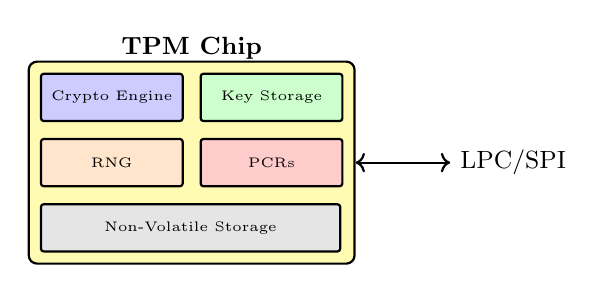
\begin{tikzpicture}[
                component/.style={draw, thick, minimum width=1.8cm, minimum height=0.6cm,
                                align=center, font=\tiny, rounded corners=1pt},
                tpm outline/.style={draw, thick, fill=yellow!30, rounded corners=3pt,
                                   inner sep=4pt}]

                % TPM internal components - position relative to each other
                \node[component, fill=blue!20] (crypto) {Crypto Engine};
                \node[component, fill=green!20, right=0.2cm of crypto] (keys) {Key Storage};
                \node[component, fill=orange!20, below=0.2cm of crypto] (rng) {RNG};
                \node[component, fill=red!20, below=0.2cm of keys] (pcr) {PCRs};
                \node[component, fill=gray!20, minimum width=3.8cm, below=0.2cm of rng.south west,
                      anchor=north west] (nvstorage) {Non-Volatile Storage};

                % TPM Chip outline using fit and background
                \begin{scope}[on background layer]
                    \node[tpm outline, fit={(crypto) (keys) (pcr) (nvstorage)},
                          label={[font=\small\bfseries, yshift=-3pt]north:TPM Chip}] (tpm) {};
                \end{scope}

                % External connection
                \draw[<->, thick] (tpm.east) -- ++(1.2cm, 0)
                    node[right, font=\small] {LPC/SPI};
            \end{tikzpicture}

            \vspace{0.3cm}
            \textbf{Use Cases:}
            \begin{itemize}
                \item BitLocker/LUKS disk encryption
                \item Measured/Secure Boot
                \item Remote attestation
                \item VPN client certificates
            \end{itemize}
        \end{column}
    \end{columns}
\end{frame}

\begin{frame}{Measured Boot with TPM}
    \begin{columns}
        \begin{column}{0.5\textwidth}
            \textbf{Platform Configuration Registers:}
            \begin{itemize}
                \item PCR0-7: BIOS/UEFI measurements
                \item PCR8-9: OS Loader configuration
                \item PCR10: IMA (Linux integrity)
                \item PCR11-15: OS-specific
                \item PCR16-23: Debug/Vendor-specific
            \end{itemize}
            
            \vspace{0.3cm}
            \textbf{PCR Extend Operation:}
            \begin{tcolorbox}[colback=gray!10]
                \small
                PCR[i] = SHA256(PCR[i] || data)
            \end{tcolorbox}
            \small Cannot directly write PCRs!
        \end{column}
        \begin{column}{0.5\textwidth}
            \textbf{Boot Measurement Chain:}
            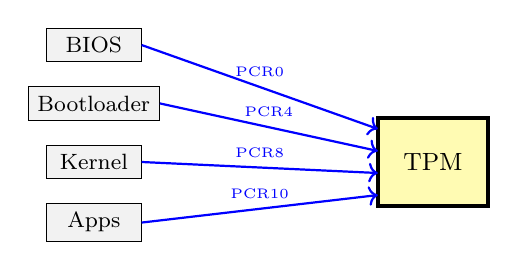
\begin{tikzpicture}[font=\footnotesize,
                component/.style={draw, fill=gray!10, minimum width=1.2cm},
                measurement/.style={->, thick, blue}]
                % Components - start with BIOS as anchor
                \node[component] (bios) {BIOS};
                \node[component, below=0.3cm of bios] (mbr) {Bootloader};
                \node[component, below=0.3cm of mbr] (kernel) {Kernel};
                \node[component, below=0.3cm of kernel] (apps) {Apps};

                % TPM as muxdemux - further right
                \node[muxdemux, muxdemux def={NL=4, Rh=2, Lh=2, w=2.5},
                      fill=yellow!30, thick, font=\small,
                      external pins width=0, right=3cm of kernel] (tpm) {TPM};

                % Measurements - straight lines to each lpin
                \draw[measurement] (bios.east) -- (tpm.lpin 1)
                    node[midway, above, font=\tiny] {PCR0};
                \draw[measurement] (mbr.east) -- (tpm.lpin 2)
                    node[midway, above, font=\tiny] {PCR4};
                \draw[measurement] (kernel.east) -- (tpm.lpin 3)
                    node[midway, above, font=\tiny] {PCR8};
                \draw[measurement] (apps.east) -- (tpm.lpin 4)
                    node[midway, above, font=\tiny] {PCR10};
            \end{tikzpicture}
            
            \vspace{0.3cm}
            \textbf{Attestation:}
            \begin{itemize}
                \item Quote = Sign(PCRs, AIK)
                \item Proves system state to remote party
                \item Unsealing secrets based on PCR values
            \end{itemize}
        \end{column}
    \end{columns}
\end{frame}

% Section 6: Summary
\section{Summary}

\begin{frame}{Hardware Security Evolution}
    \begin{center}
    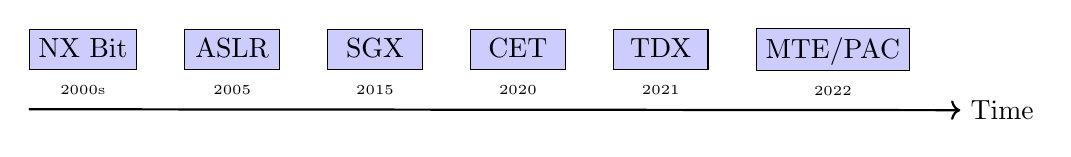
\begin{tikzpicture}[scale=0.8,
            timeline label/.style={font=\tiny, text depth=0.25ex},
            feature/.style={draw, fill=blue!20, minimum width=1.2cm, minimum height=0.5cm, text depth=0.25ex}]

            % Security features with consistent style
            \node[feature] (nx) at (1,0) {NX Bit};
            \node[timeline label, below=2pt of nx] (year-nx) {2000s};

            \node[feature, right=0.6cm of nx] (aslr) {ASLR};
            \node[timeline label, below=2pt of aslr] {2005};

            \node[feature, right=0.6cm of aslr] (sgx) {SGX};
            \node[timeline label, below=2pt of sgx] {2015};

            \node[feature, right=0.6cm of sgx] (cet) {CET};
            \node[timeline label, below=2pt of cet] {2020};

            \node[feature, right=0.6cm of cet] (tdx) {TDX};
            \node[timeline label, below=2pt of tdx] {2021};

            \node[feature, right=0.6cm of tdx] (mte) {MTE/PAC};
            \node[timeline label, below=2pt of mte] (year-mte) {2022};

            % Timeline arrow (positioned relative to nodes)
            \draw[thick,->] ([yshift=-1pt]nx.west |- year-nx.south) -- ([yshift=-1pt, xshift=0.8cm]mte.east |- year-mte.south) node[right] {Time};
        \end{tikzpicture}
    \end{center}

    \vspace{0.3cm}
    \begin{columns}
        \begin{column}{0.5\textwidth}
            \textbf{Current Trends:}
            \begin{itemize}
                \item Hardware-software co-design
                \item Confidential computing
                \item Memory safety focus
                \item Supply chain security
            \end{itemize}
        \end{column}
        \begin{column}{0.5\textwidth}
            \textbf{Challenges:}
            \begin{itemize}
                \item Performance overhead
                \item Compatibility issues
                \item Side-channel attacks
                \item Ecosystem adoption
            \end{itemize}
        \end{column}
    \end{columns}
\end{frame}

\begin{frame}{Key Takeaways}
    \begin{itemize}
        \item \textbf{Defense in Depth:} Multiple layers of security mechanisms
        \vspace{0.3cm}
        \item \textbf{Hardware Acceleration:} Critical security features need hardware support for performance
        \vspace{0.3cm}
        \item \textbf{Trust Boundaries:} Clear separation between trusted and untrusted components
        \vspace{0.3cm}
        \item \textbf{Attestation:} Cryptographic proof of system state and configuration
        \vspace{0.3cm}
        \item \textbf{Memory Protection:} Tags, authentication, and encryption for memory safety
        \vspace{0.3cm}
        \item \textbf{Control Flow:} Hardware enforcement of valid program execution paths
    \end{itemize}
    
    \vspace{0.5cm}
    \begin{tcolorbox}[colback=blue!20]
        \centering
        \textbf{Future:} Homomorphic encryption, quantum-resistant crypto, AI-driven security
    \end{tcolorbox}
\end{frame}

\end{document}